
\begin{frame}
  \begin{center}
    \large{1. Machines à vecteurs de support (SVM)}
  \end{center}
\end{frame}

\begin{frame}{1.1 SVM: le principe}
  \begin{figure}[htb]
    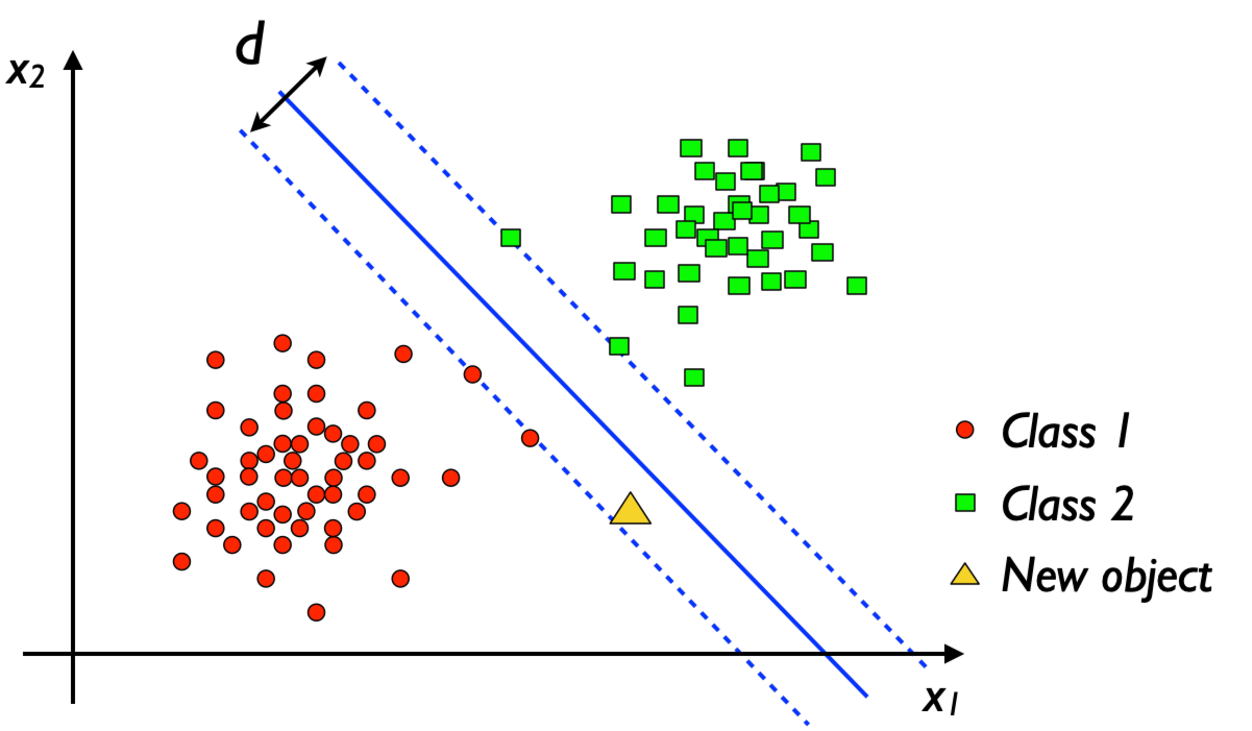
\includegraphics[width=0.5\textwidth]{figures/SVM_general.pdf}
  \end{figure}
  \begin{itemize}
    \item On considère des données linéairement séparables.
    \item Un jeu de données $\dset = \{(\xvec_1, y_1), (\xvec_2, y_2), \dots, (\xvec_n, y_n)\}$ avec $y_i \in \{-1, 1\}$ est linéairement séparable, s'il existe un hyperplan tel que toutes les données avec $y_i=-1$ se trouvent d'un côté de l'hyperplan et toutes les données avec $y_i=1$ de l'autre. 
  \end{itemize}
\end{frame}

\begin{frame}{1.1 SVM: le principe}
  \begin{figure}[htb]
    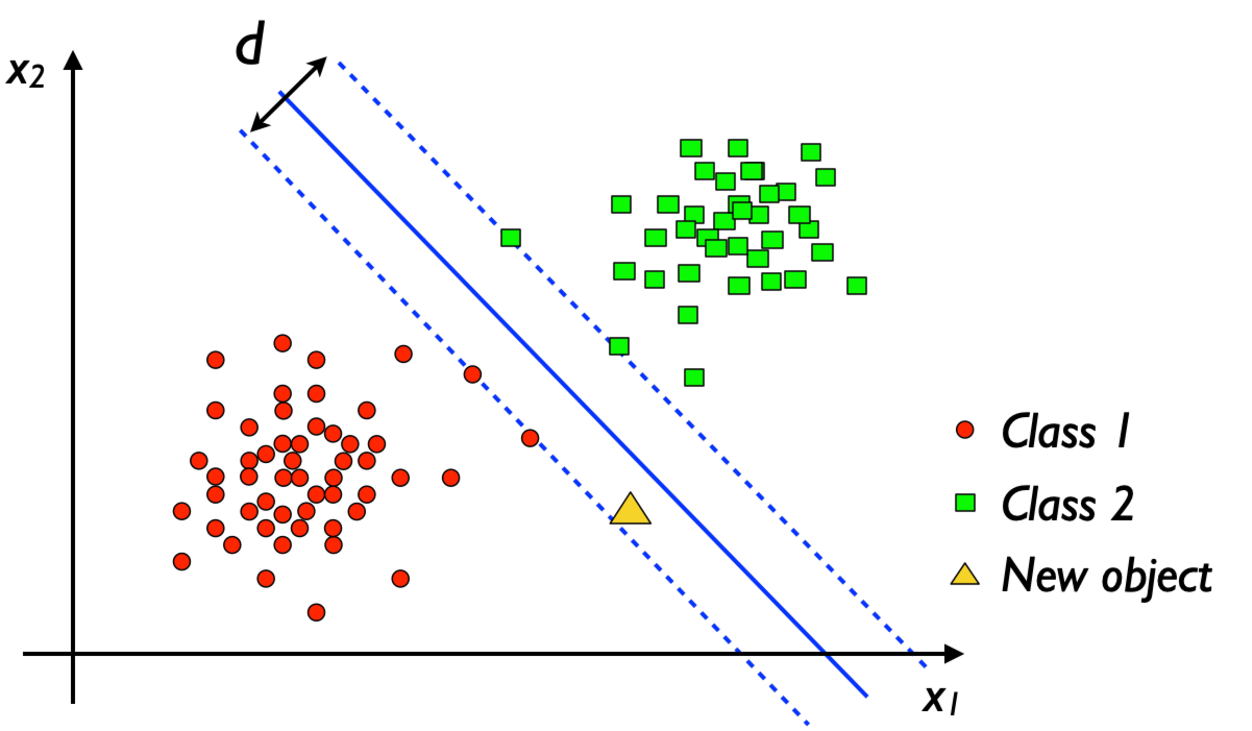
\includegraphics[width=0.5\textwidth]{figures/SVM_general.pdf}
  \end{figure}
  \begin{itemize}
    \item Pour des données linéairement séparables, on place un "ruban" entre les données, c'est-à-dire un hyperplan avec ces deux parallèles $h^+$ et $h^-$. 
    \item On appelle $d$ la distance entre $h^+$ et $h^-$ la marge du classifieur. 
    \item Les "classifieurs à large marge" visent à maximiser $d$. 
  \end{itemize}
\end{frame}

\begin{frame}{1.2 SVM: le cas séparable}
  \begin{figure}[htb]
    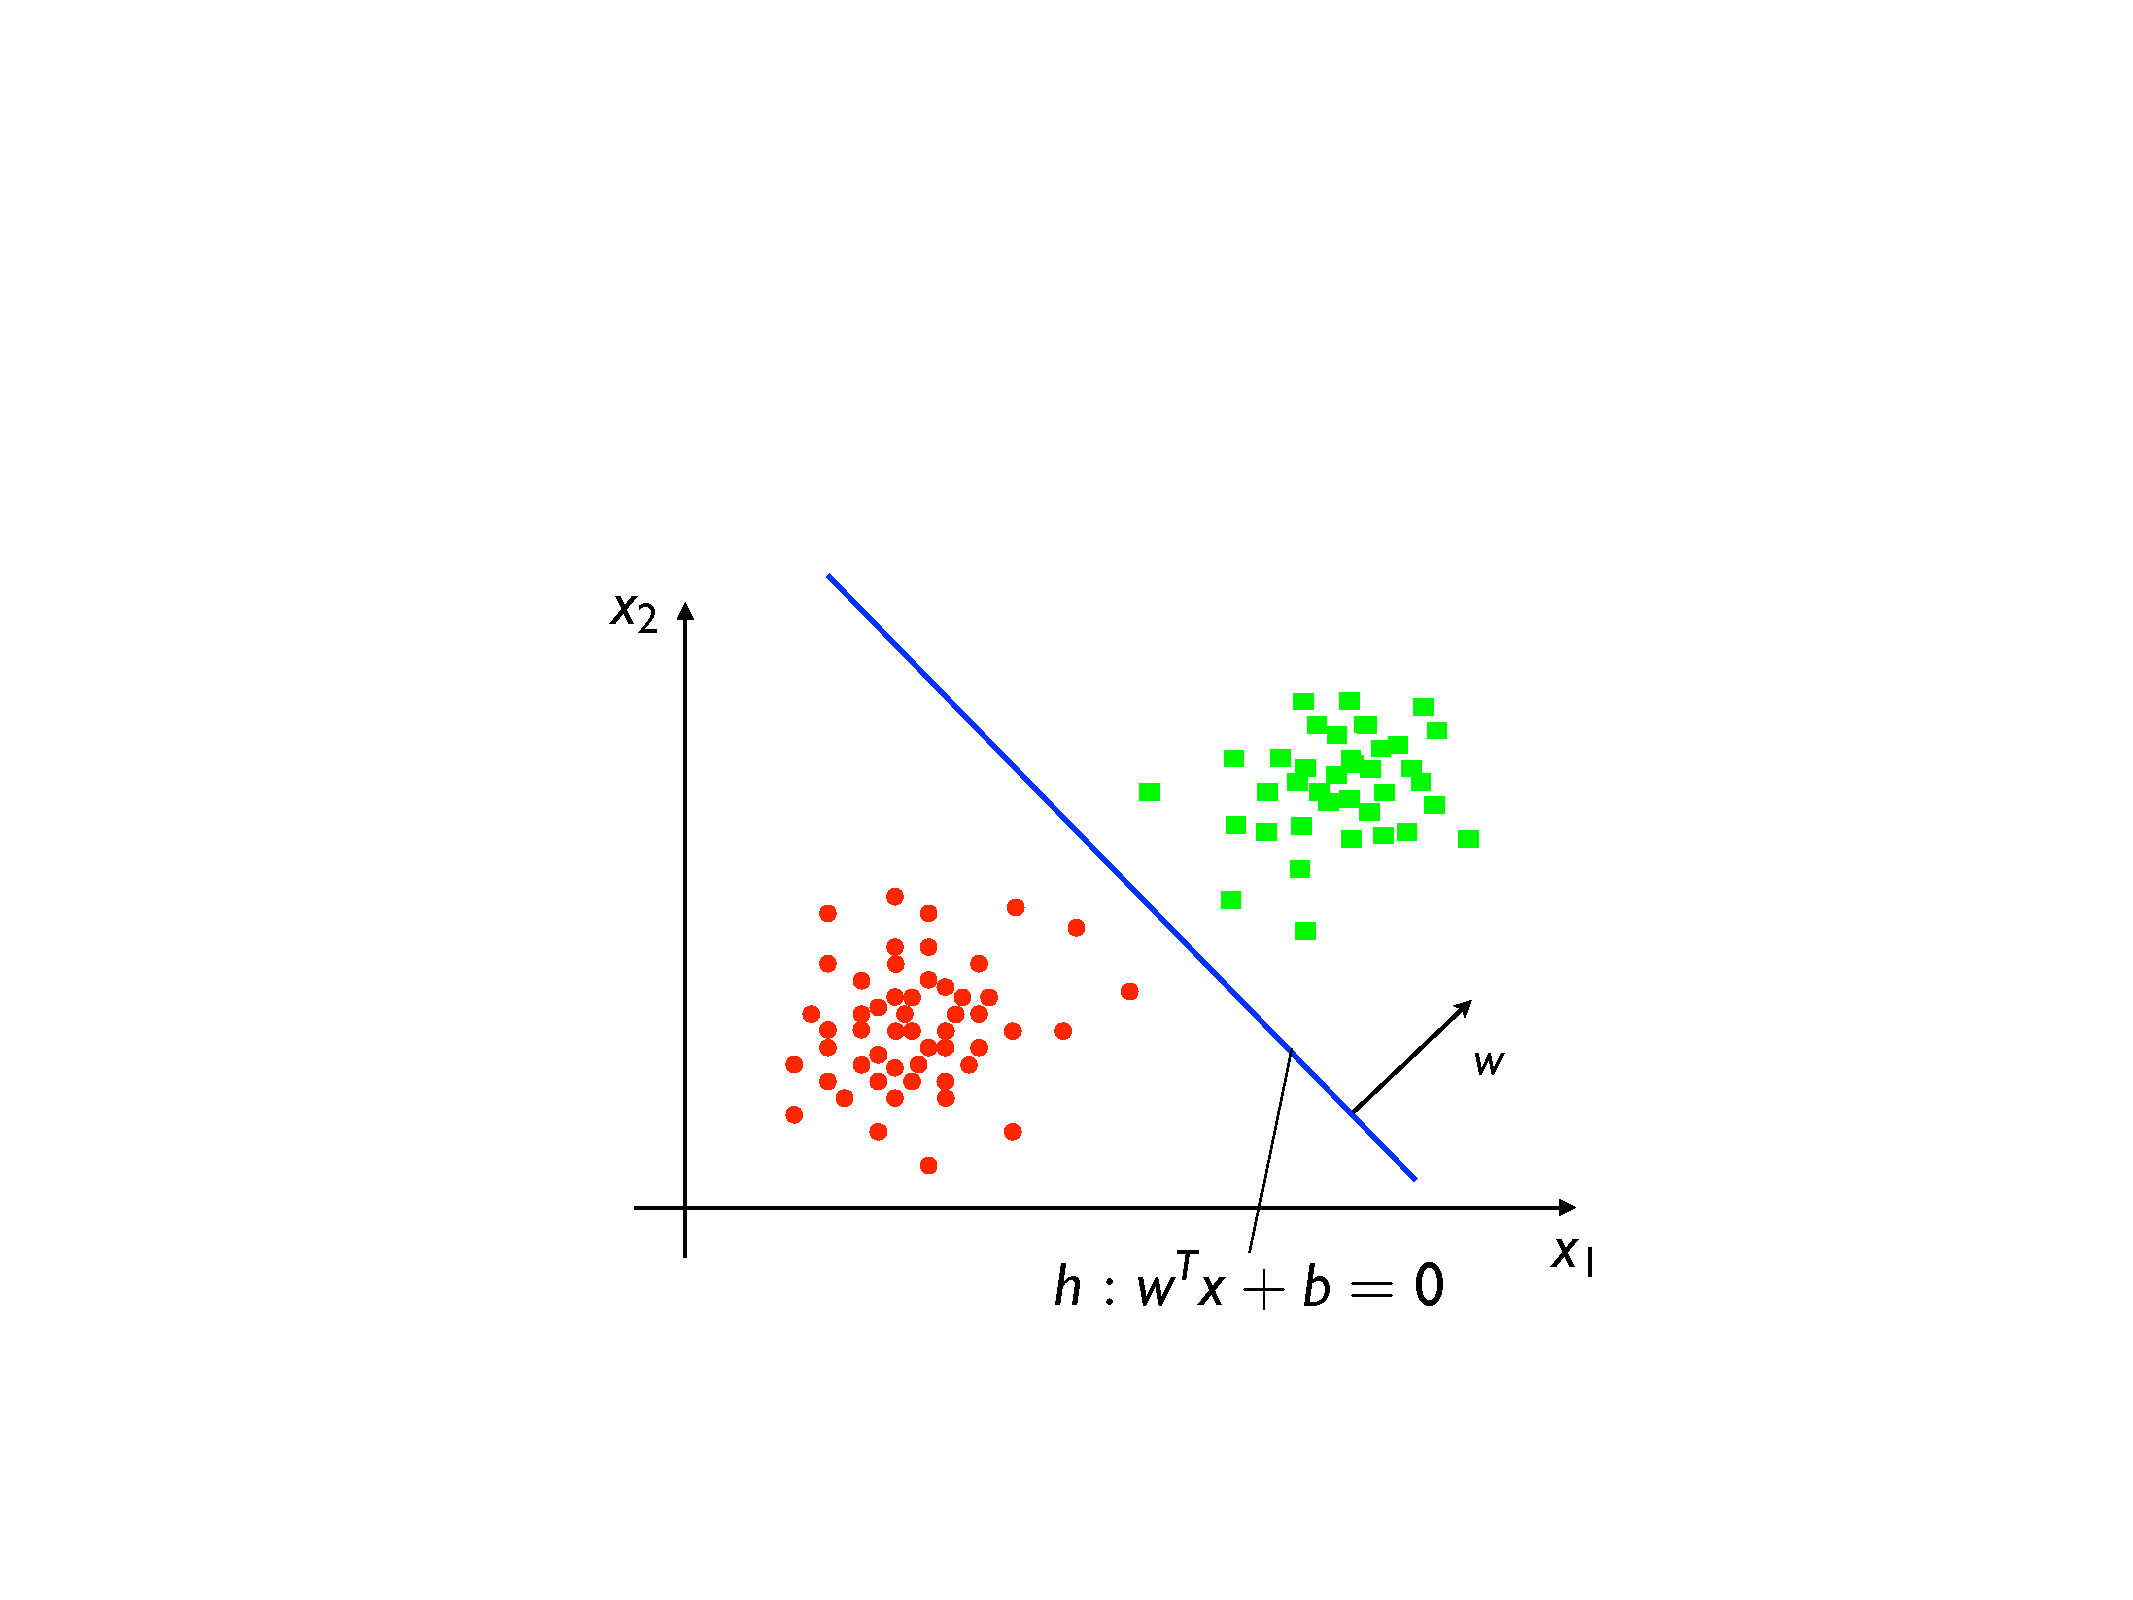
\includegraphics[width=0.6\textwidth]{figures/SVM_1a.pdf}
  \end{figure}
  \begin{itemize}
    \item Hyperplan séparateur $h: \langle \overrightarrow{w};\overrightarrow{x} \rangle + b = 0$.
    \item $\overrightarrow{w}$: vecteur normal de l'hyperplan séparateur. $b$ est le biais (intercept). 
    \item $\langle\overrightarrow{w};\overrightarrow{x} \rangle$ est le produit scalaire du vecteur normal (vecteur des poids) avec le vecteur des descripteurs. 
    \item Pour des descripteurs centrés réduits, $\overrightarrow{w}$ reflète l'importance des descripteurs.
  \end{itemize}
\end{frame}

\begin{frame}{1.2 SVM: le cas séparable}
  \begin{figure}[htb]
    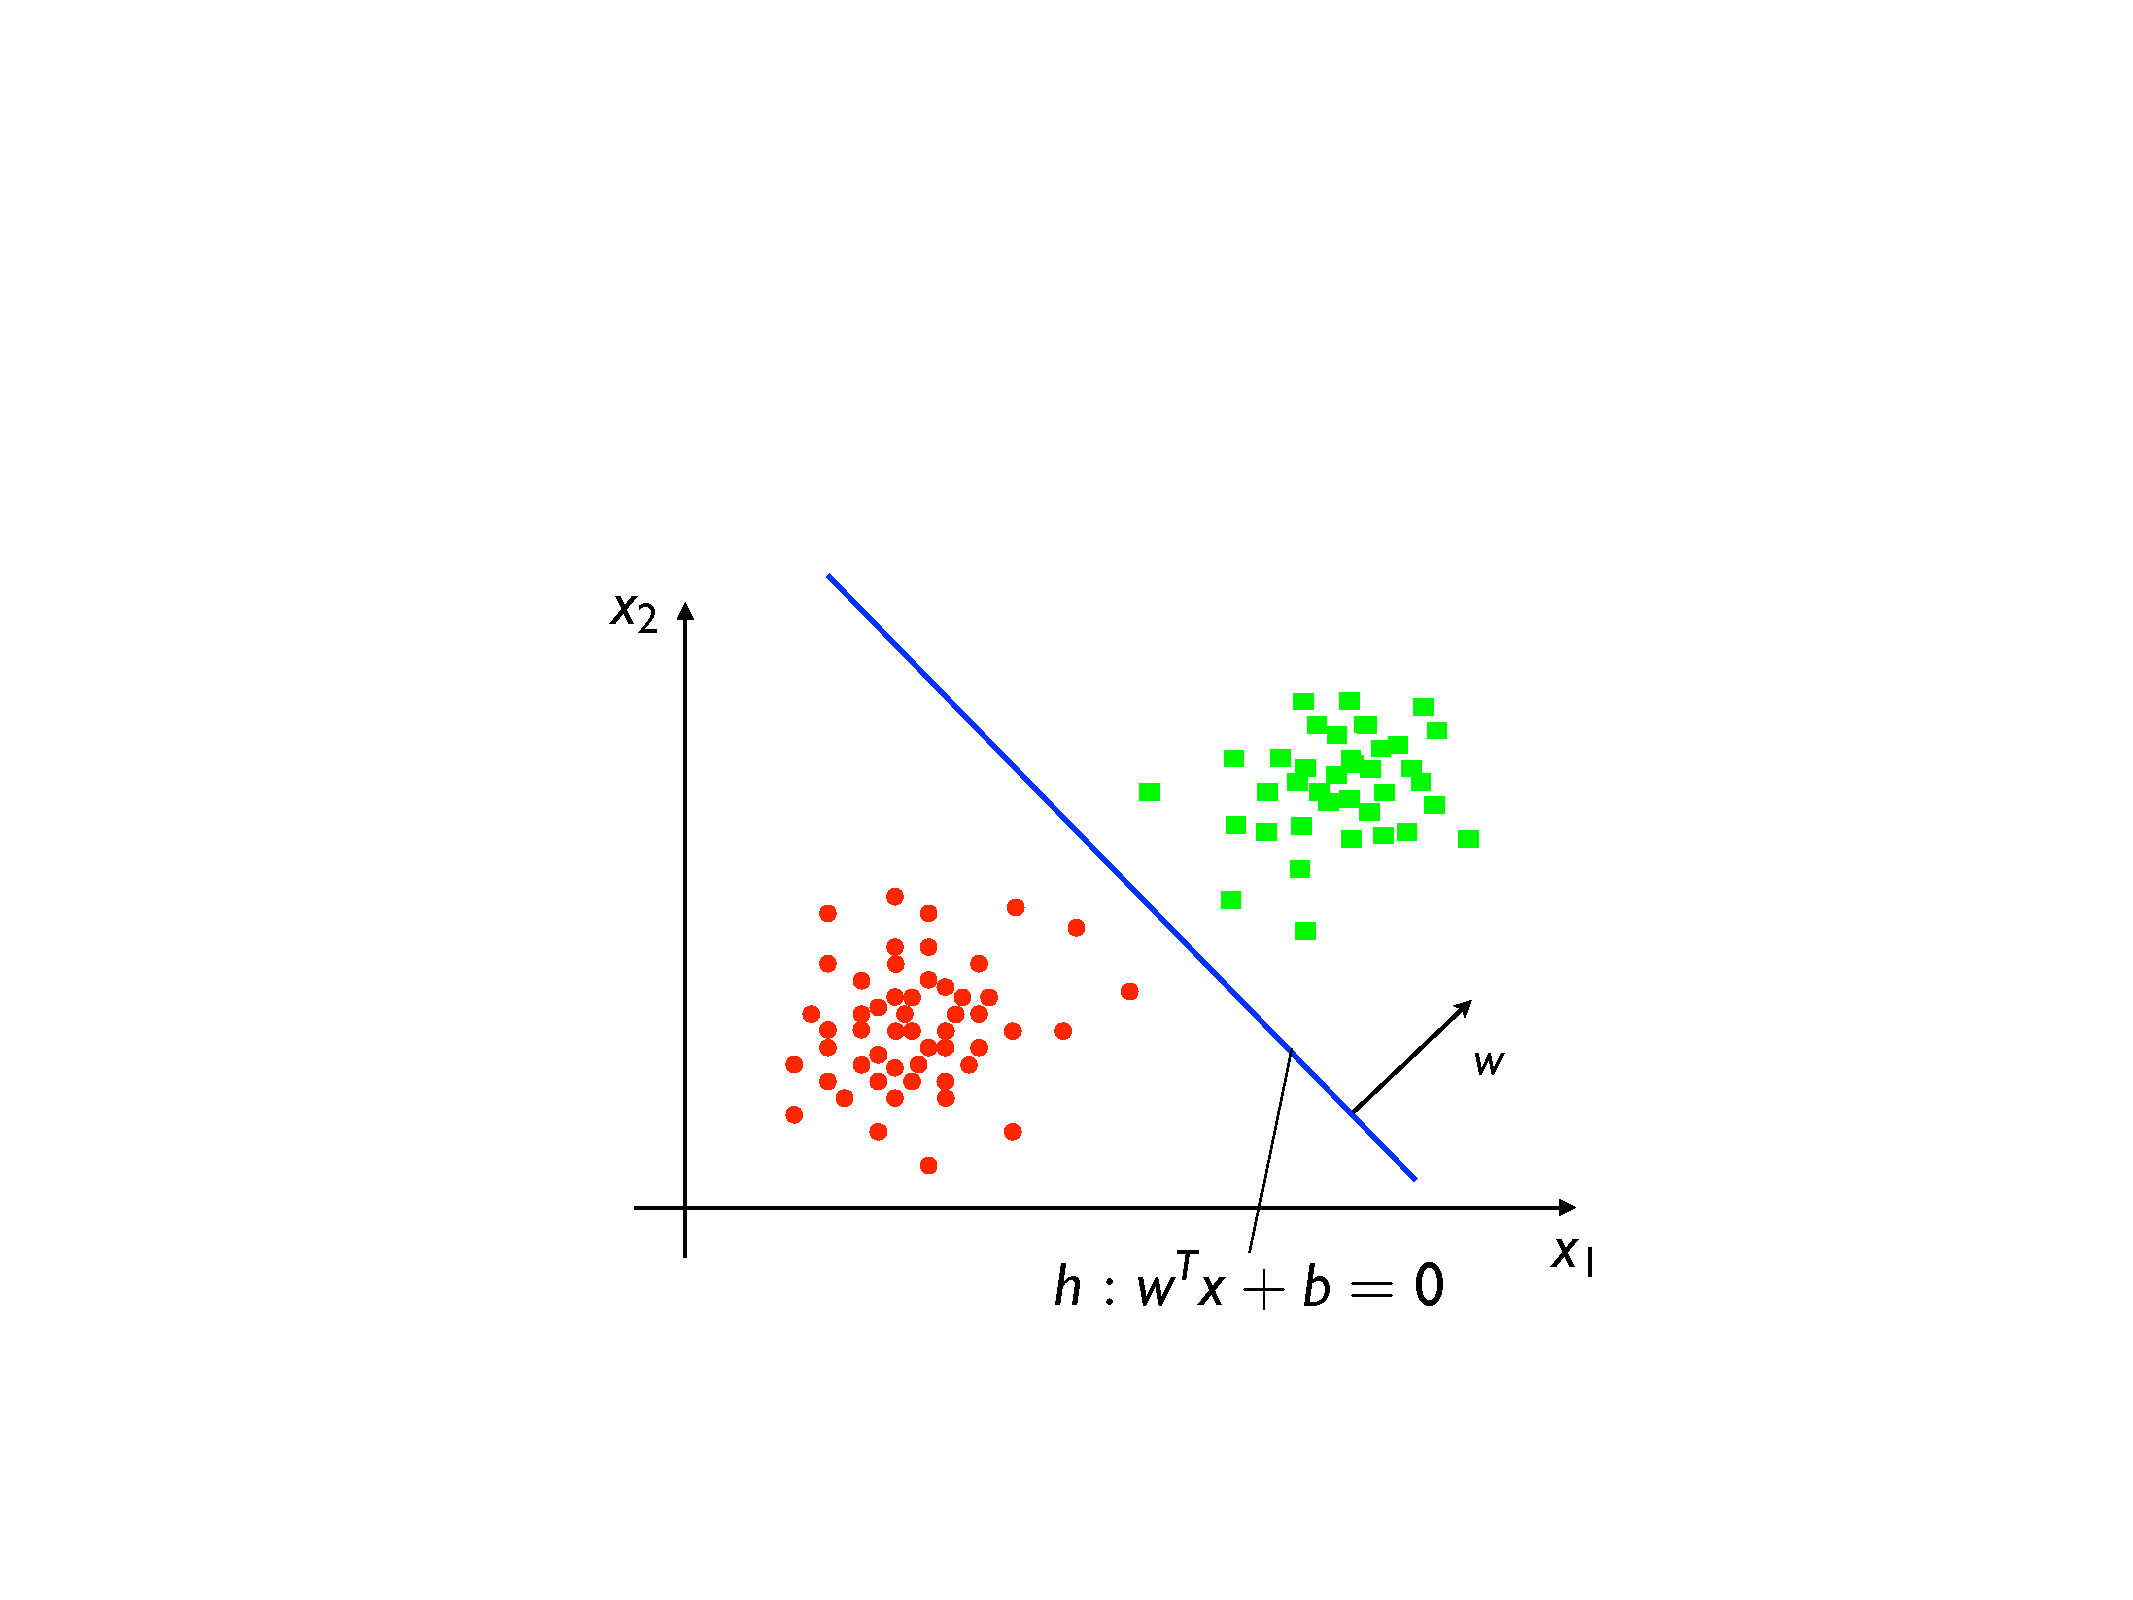
\includegraphics[width=0.6\textwidth]{figures/SVM_1a.pdf}
  \end{figure}
  \begin{itemize}
    \item $\langle\overrightarrow{w},\overrightarrow{x} \rangle + b  > 0$: $\overrightarrow{x}$ se trouve du côté vers lequel $\overrightarrow{w}$ pointe. 
    \item $\langle \overrightarrow{w}, \overrightarrow{x} \rangle + b  < 0$: $\overrightarrow{x}$ se trouve du côté opposé. 
    \item Avec l'encodage $y\in\{-1,+1\}$, un échantillon $\overrightarrow{x_i}$ est correctement classifié si $y_i(\langle \overrightarrow{w};\overrightarrow{x_i} \rangle + b) > 0$.
  \end{itemize}
\end{frame}

\begin{frame}{1.2 SVM: le cas séparable}
  \begin{figure}[htb]
    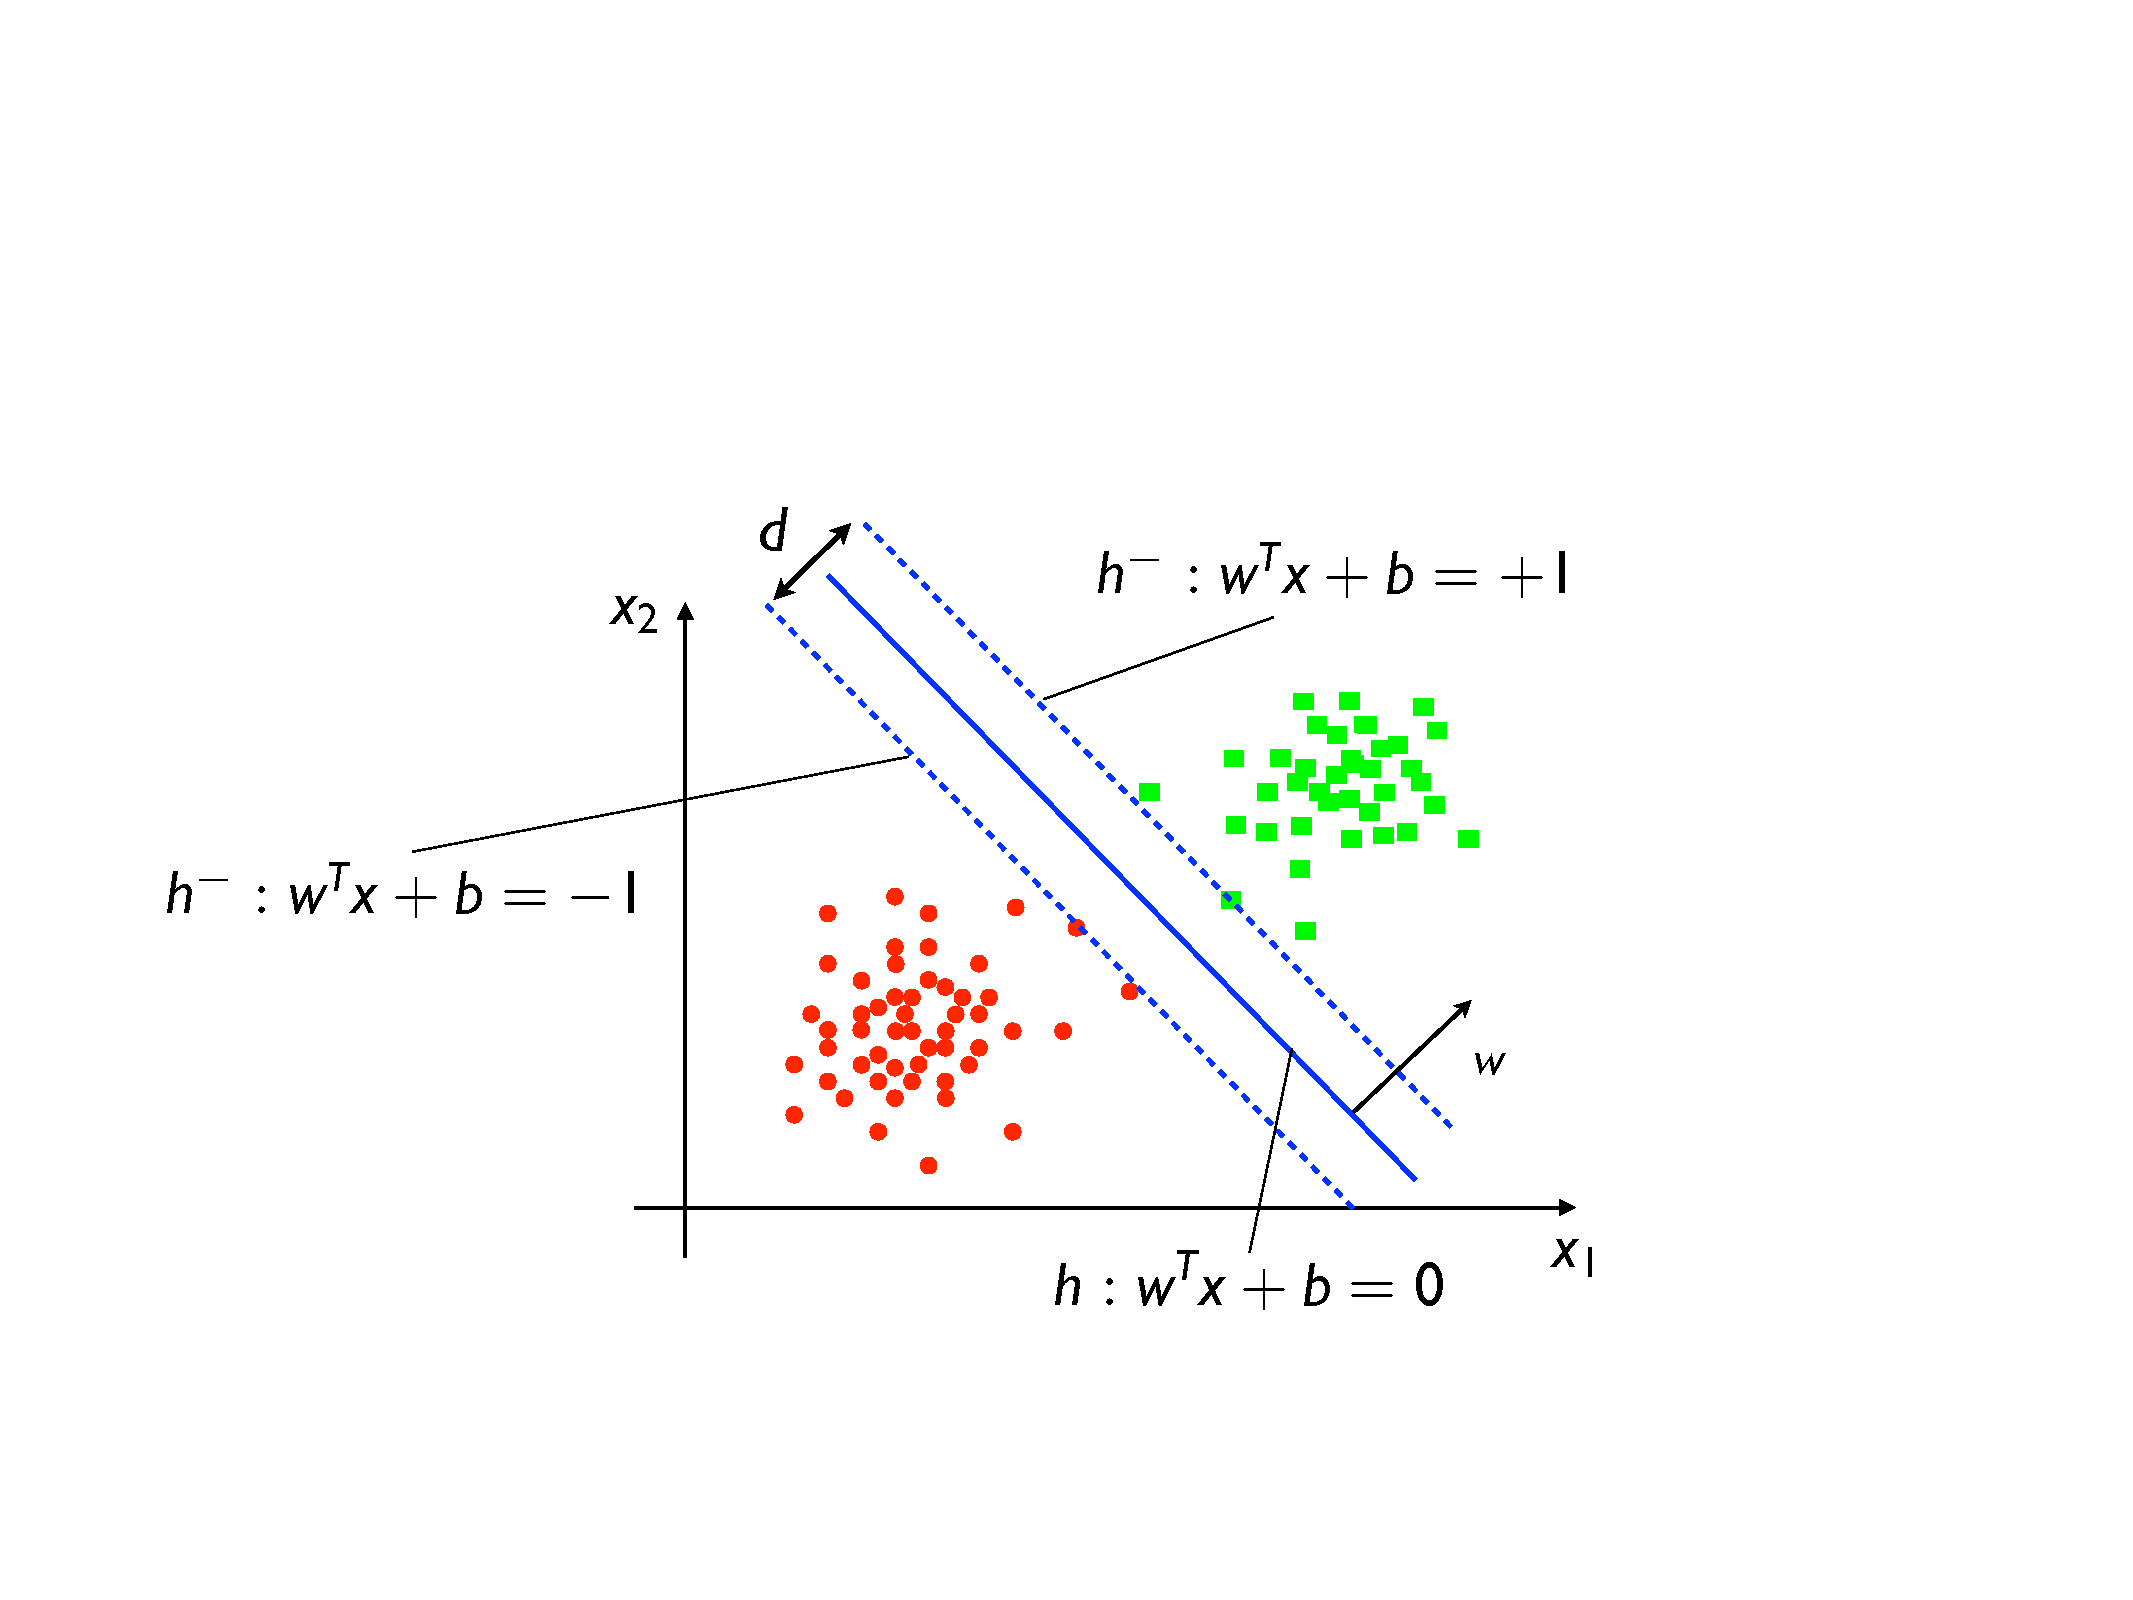
\includegraphics[width=0.6\textwidth]{figures/SVM2.pdf}
  \end{figure}
  \begin{itemize}
    \item Le ruban est défini par deux hyperplans parallèles, pour lesquels $\langle \overrightarrow{w};\overrightarrow{x} \rangle + b = \pm 1$ 
    \item La distance entre ces deux hyperplans $\langle \overrightarrow{w};\overrightarrow{x} \rangle + b = \pm 1$ est : 
    \begin{equation}
      d = \frac{2}{\|\overrightarrow{w}\|}
    \end{equation}
    \item Maximiser $d$ est équivalent à minimiser $\|\overrightarrow{w}\|^2$.
  \end{itemize}
\end{frame}


% \begin{frame}{1.2 SVM: le cas séparable}
%   \begin{figure}[htb]
%     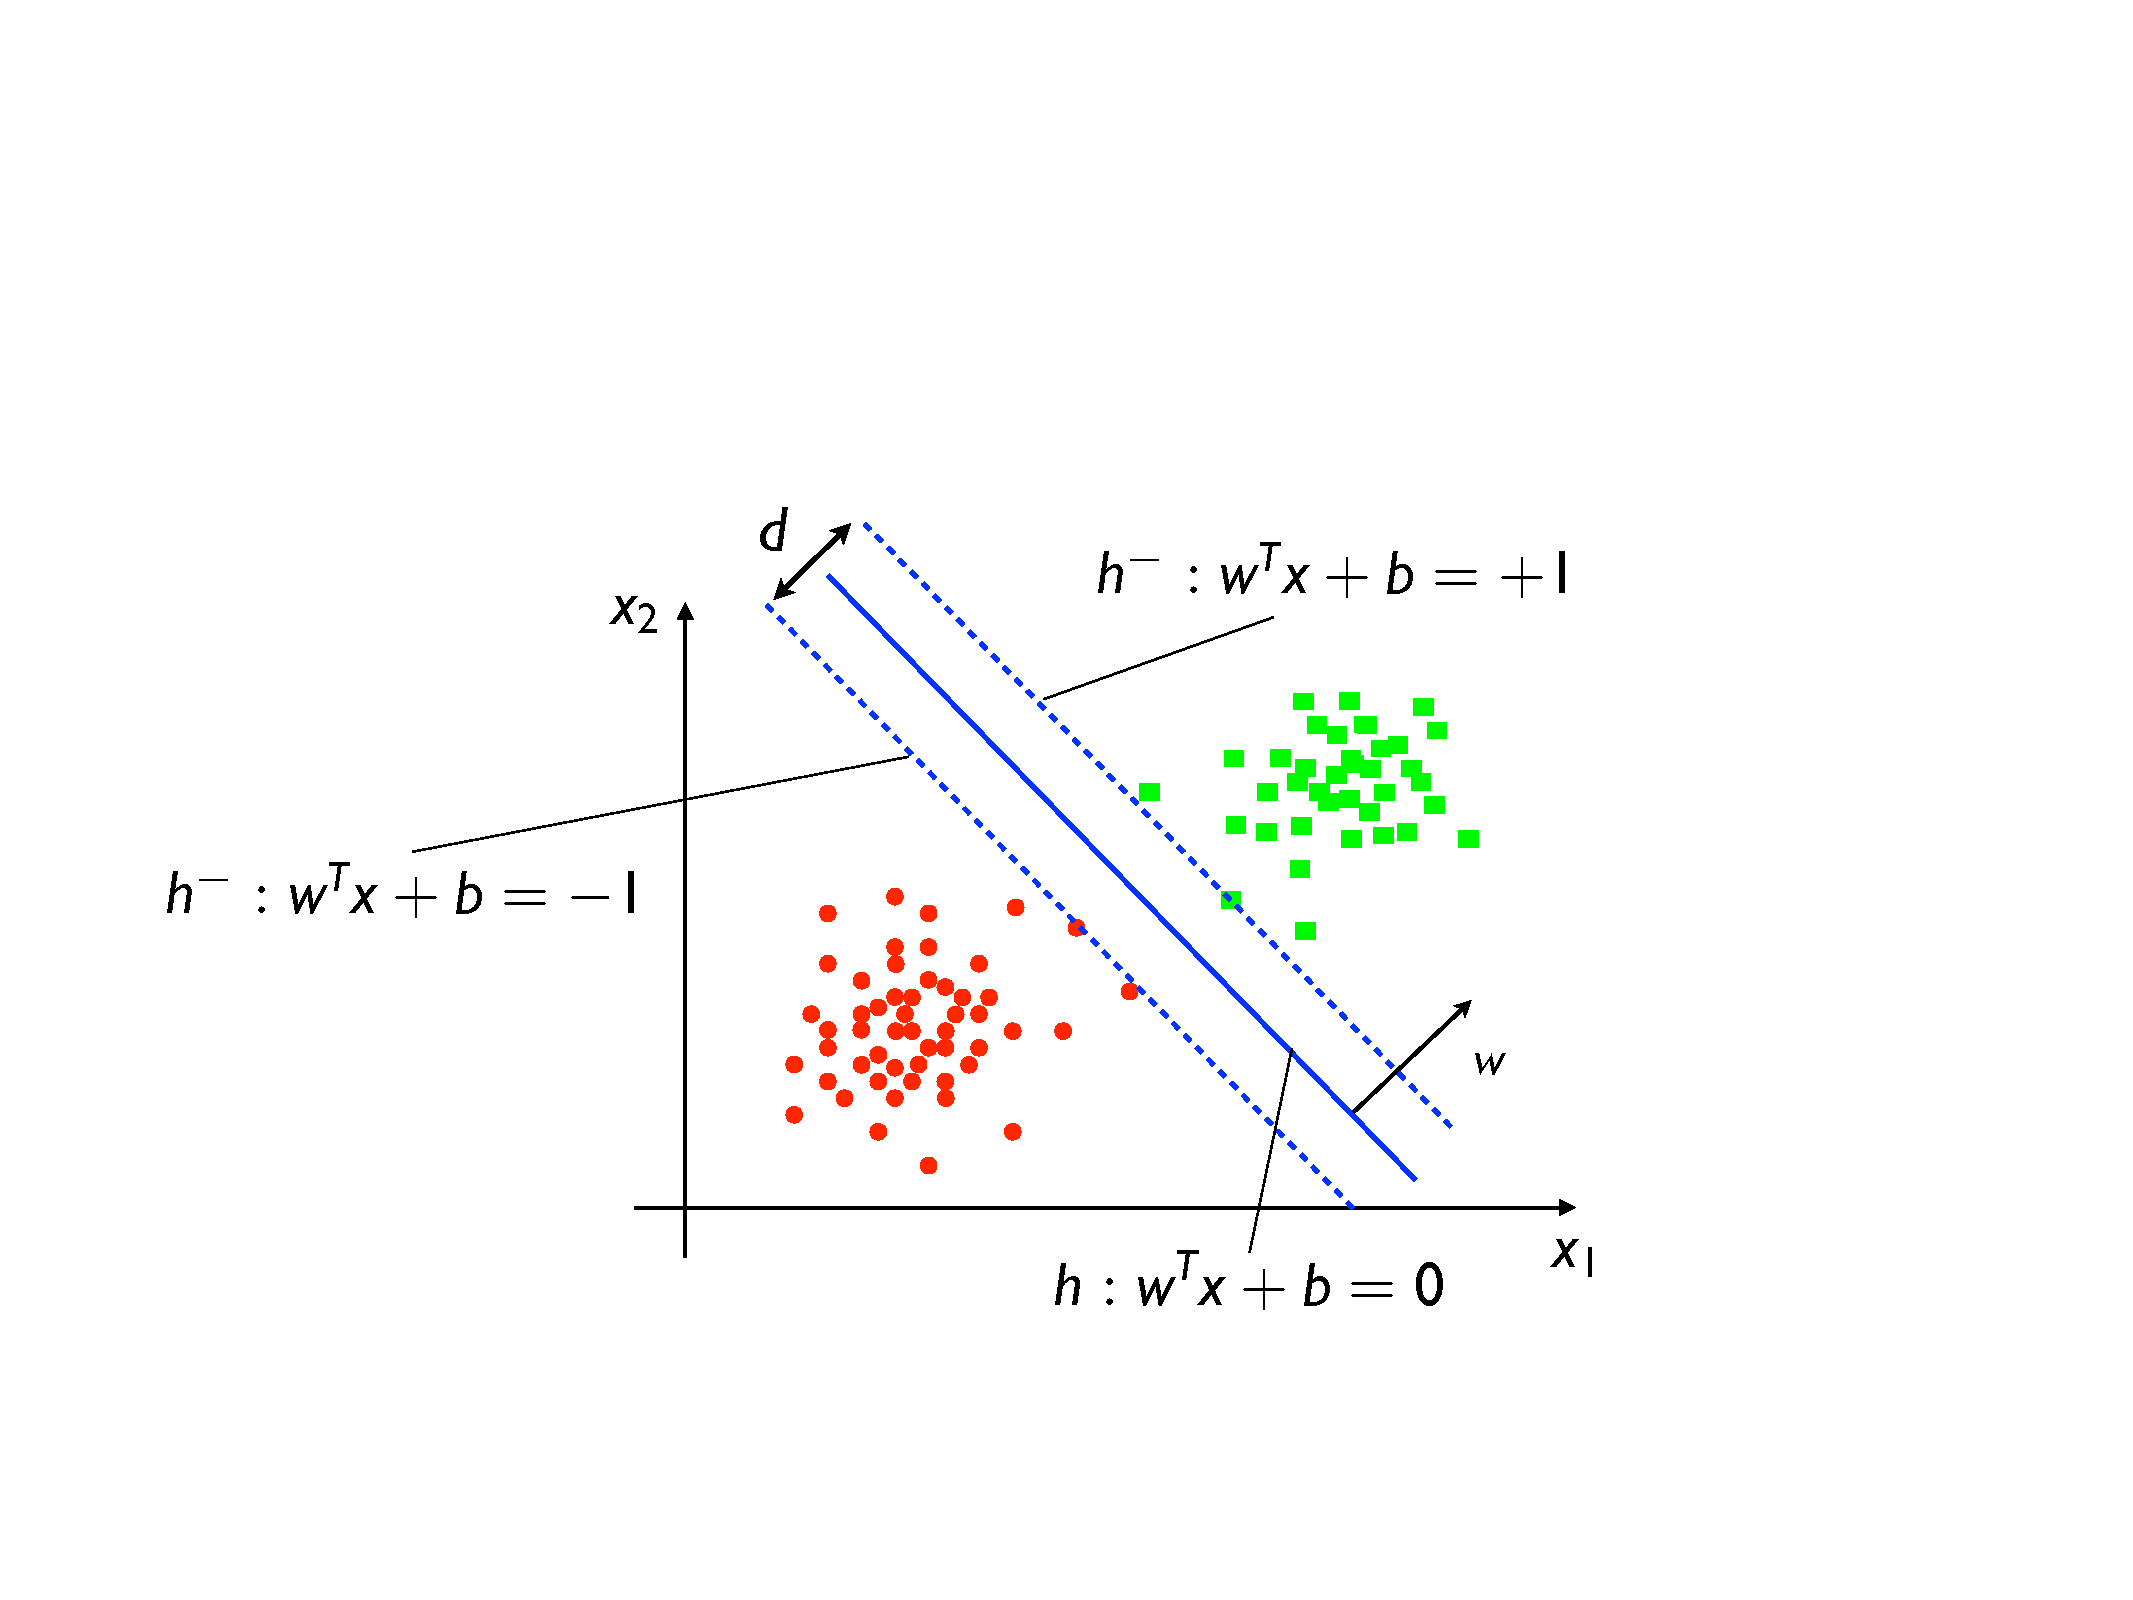
\includegraphics[width=0.6\textwidth]{figures/SVM2.pdf}
%   \end{figure}
%   \begin{itemize}
%     \item Cela mène à un problème d'\textbf{optimisation convexe sous contraintes} : 
%     \begin{eqnarray*}
%       \mbox{minimize} & & \|\overrightarrow{w}\|^2 \\
%       \mbox{subject to} & & y_i(\langle \overrightarrow{w};\overrightarrow{x_i} \rangle + b) \geq 1 \quad i = 1, \ldots, N
%     \end{eqnarray*}
%     \item La convexité implique qu'il n'y a pas de minimum local en dehors du minimum global. 
%   \end{itemize}
% \end{frame}


\begin{frame}{1.2 SVM: le cas séparable}
  \begin{figure}[htb]
    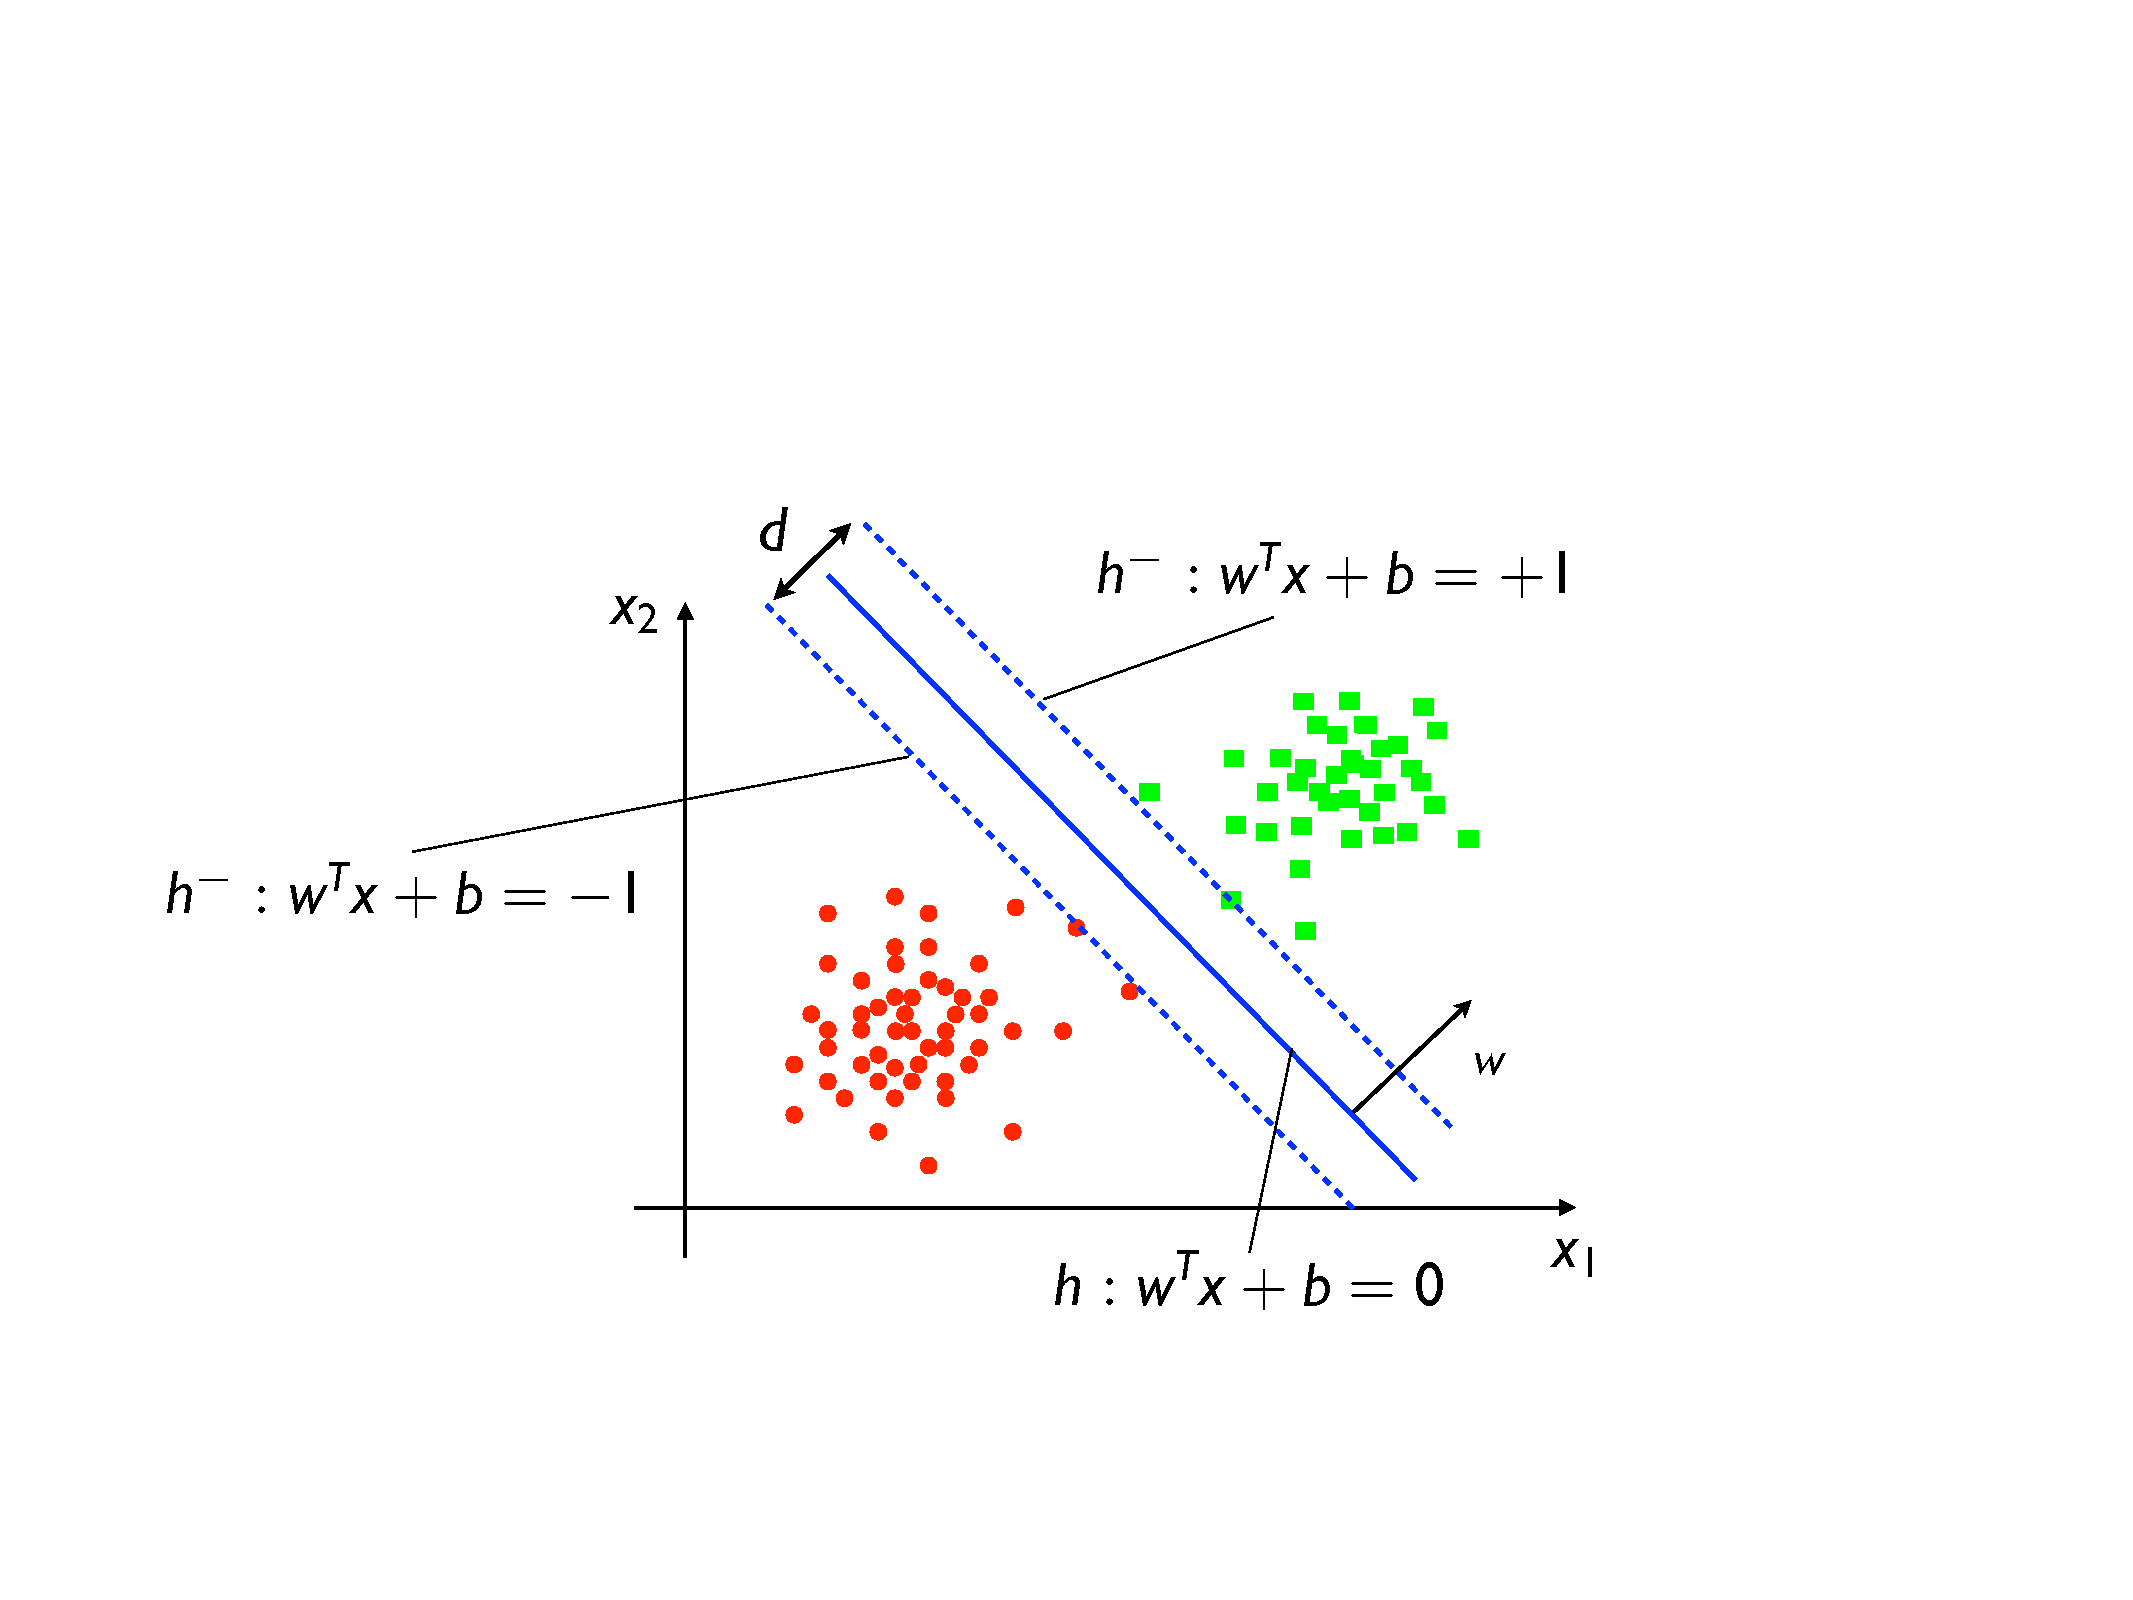
\includegraphics[width=0.6\textwidth]{figures/SVM2.pdf}
  \end{figure}
  \begin{itemize}
    \item Cela mène à un problème d'\textbf{optimisation convexe sous contraintes} : 
    \begin{eqnarray*}
      \min & & \frac{1}{2}\|\overrightarrow{w}\|^2 \\
      \mbox{t.q.} & & y_i(\langle \overrightarrow{w};\overrightarrow{x_i} \rangle + b) \geq 1 \quad i = 1, \ldots, N
    \end{eqnarray*}
    \item La convexité implique que chaque minimum local est aussi minimum global. 
  \end{itemize}
\end{frame}

\begin{frame}{1.2 SVM: le cas séparable}
\begin{itemize}
  \item La solution de ce problème d'optimisation et notée $\wvec^{\ast},b^{\ast}$ et définit la fonction de décision optimale : 
  \begin{equation}
    f(\xvec) = \langle \wvec^\ast, \xvec \rangle + b^\ast.
  \end{equation}
  \item Introduction des multiplicateurs de Lagrange $\alpha_i \geq 0$, un par contrainte.
  \begin{equation}
    \mathcal{L}(\wvec, b, \alphavec) =
      \frac{1}{2} \|\wvec\|_2^2
      - \sum_{i=1}^n \alpha_i
      \Bigl( y_i (\langle \wvec, \xvec_i \rangle + b) - 1 \Bigr).
  \end{equation}
  \item Il est facile de comprendre que $\min_{\wvec,b}{\mathcal{L}(\wvec, b, \alphavec)}\leq\|\wvec^*\|^2$ si $\alpha_i \geq 0 \; \forall i$, puisqu'on soustrait des termes non-négatifs. 
\end{itemize}
%  En minimisant $\mathcal{L}$ par rapport à $\bm{w}$ et $b$, puis en maximisant par rapport à $\bm{\alpha}$,
 % on obtient le \textbf{problème dual}.
\end{frame}

\begin{frame}{1.2 SVM: le cas séparable}
\begin{itemize}
  \item On minimise $\mathcal{L}(\wvec,b,\alphavec)$ par rapport à $\wvec$ et $b$ en mettant les dérivées partielles à 0: 
\begin{eqnarray*}
\frac{\partial \mathcal{L}(\wvec,b,\alphavec)}{\partial \wvec} &=& \wvec - \sum_{i=1}^{N} \alpha_iy_i\xvec_i = 0 \quad \Rightarrow \quad \wvec = \sum_{i=1}^{N} \alpha_iy_i\xvec_i\\
\frac{\partial \mathcal{L}(\wvec,b,\alphavec)}{\partial b} &=& - \sum_{i=1}^{N} y_i\alpha_i = 0 \quad \Rightarrow \quad \sum_{i=1}^{N} y_i\alpha_i = 0
\end{eqnarray*}
\item On obtient alors : $g(\alphavec)=\min_{\wvec,b}\mathcal{L}(\wvec, b, \alphavec)$: 
\begin{equation*}
g(\alphavec) = \sum_{i=1}^{N}\alpha_i - \frac{1}{2}\sum_{i=1}^N\sum_{j=1}^N\alpha_i\alpha_jy_iy_j\langle\xvec_i \xvec_j\rangle
\end{equation*}
\end{itemize}
\end{frame}

\begin{frame}{1.2 SVM: le cas séparable}
\begin{itemize}
  \item Par construction, nous savons que $g(\alphavec)\leq\frac{1}{2}\|\wvec^\ast\|^2$ (on rappelle que $\wvec^\ast$ 
  est la solution du problème d'optimisation sous contraintes). 
  \item Si maintenant on maximise par rapport à $\alphavec$ (sous contraintes $\sum_{i=1}^{N} y_i\alpha_i = 0$ and $\alpha_i\geq 0$)), on obtient la meilleure borne inférieure et - dans ce cas - $g(\alphavec^\ast)=\frac{1}{2}\|\wvec^\ast\|^2$.

\end{itemize}
\end{frame}

\begin{frame}{1.2 SVM: le cas séparable}
\begin{itemize}
\item Au lieu de résoudre le problème d'optimisation convexe sous contraintes, on résoudra alors le problème dual : 
\begin{eqnarray*}
 &\max_{\alphavec}& g(\alphavec) = \sum_{i=1}^{N}\alpha_i - \frac{1}{2}\sum_{i=1}^N\sum_{j=1}^N\alpha_i\alpha_jy_iy_j\langle\xvec_i,\xvec_j\rangle \\
&\mbox{t.q.}& \alpha_i \geq 0 \, \forall i \\
&\, & \sum_{i=1}^N\alpha_iy_i=0
\end{eqnarray*}
\end{itemize}
\end{frame}

\begin{frame}{1.2 SVM: le cas séparable}
\begin{itemize}
\item On suppose que $\wvec^\ast$ est une solution du problème primal et $\alphavec^\ast$ une solution du problème dual. Alors :  
\begin{eqnarray*}
f(\wvec^\ast) &=& g(\alphavec^\ast)\\
&=& \inf_{\wvec,b}\mathcal{L}(\wvec,\alphavec^\ast, b)\\
&\leq & f(\wvec^\ast) - \sum_{i=1}^N\alpha_i^*(y_i(\langle\wvec^{\ast},\xvec_i\rangle+b^\ast)-1)\\
&\leq & f(\wvec^\ast)
\end{eqnarray*}
\item Donc: $\forall i \, \, \alpha_i^*(y_i(\langle\wvec^\ast,\xvec\rangle+b^\ast)-1) = 0$. 
\begin{itemize}
\item $\alpha_i^\ast=0$: $\xvec_i$ n'est pas sur un hyperplan parallèle. 
\item $\alpha_i^\ast\neq 0$: $\xvec_i$ est sur un hyperplan parallèle, la conditions est "active" ($\xvec_i$ est un vecteur de support). 
\end{itemize}
\end{itemize}
\end{frame}


\begin{frame}{1.2 SVM: le cas séparable}
\begin{itemize}
\item On rappelle la solution $\wvec^\ast$ du problème primal: 
\begin{equation*}
\wvec^\ast = \sum_{i=1}^{N}\alpha_iy_i\xvec_i
\end{equation*}
\item $\wvec^\ast$ est donc la somme pondérée des instances $\xvec_i$ pour lesquels $\alpha_i \neq 0$ (vecteurs de support).
\item La solution pour l'hyperplan séparateur est donc : 
\begin{eqnarray*}
f(\xvec) &=& \langle\wvec, \xvec\rangle + b \\ 
&=& \sum_{i=1}^N\alpha_iy_i\langle\xvec_i,\xvec\rangle + b \\
&=& \sum_{i\in SV}\alpha_iy_i\langle\xvec_i,\xvec\rangle + b
\end{eqnarray*}
où $SV$ est l'ensemble des vecteurs support. 
%L'hyperplan dépend uniquement de produits scalaires de $\xvec$ avec les vecteurs de support $\xvec_i$. 
\end{itemize}
\end{frame}



%%%%%%%%%%%%%%%%%%%%%%%%%%%%%%%%%%%%%%%%%%

\begin{frame}{1.3 SVM pour le cas non-séparable}
  \begin{figure}[htb]
    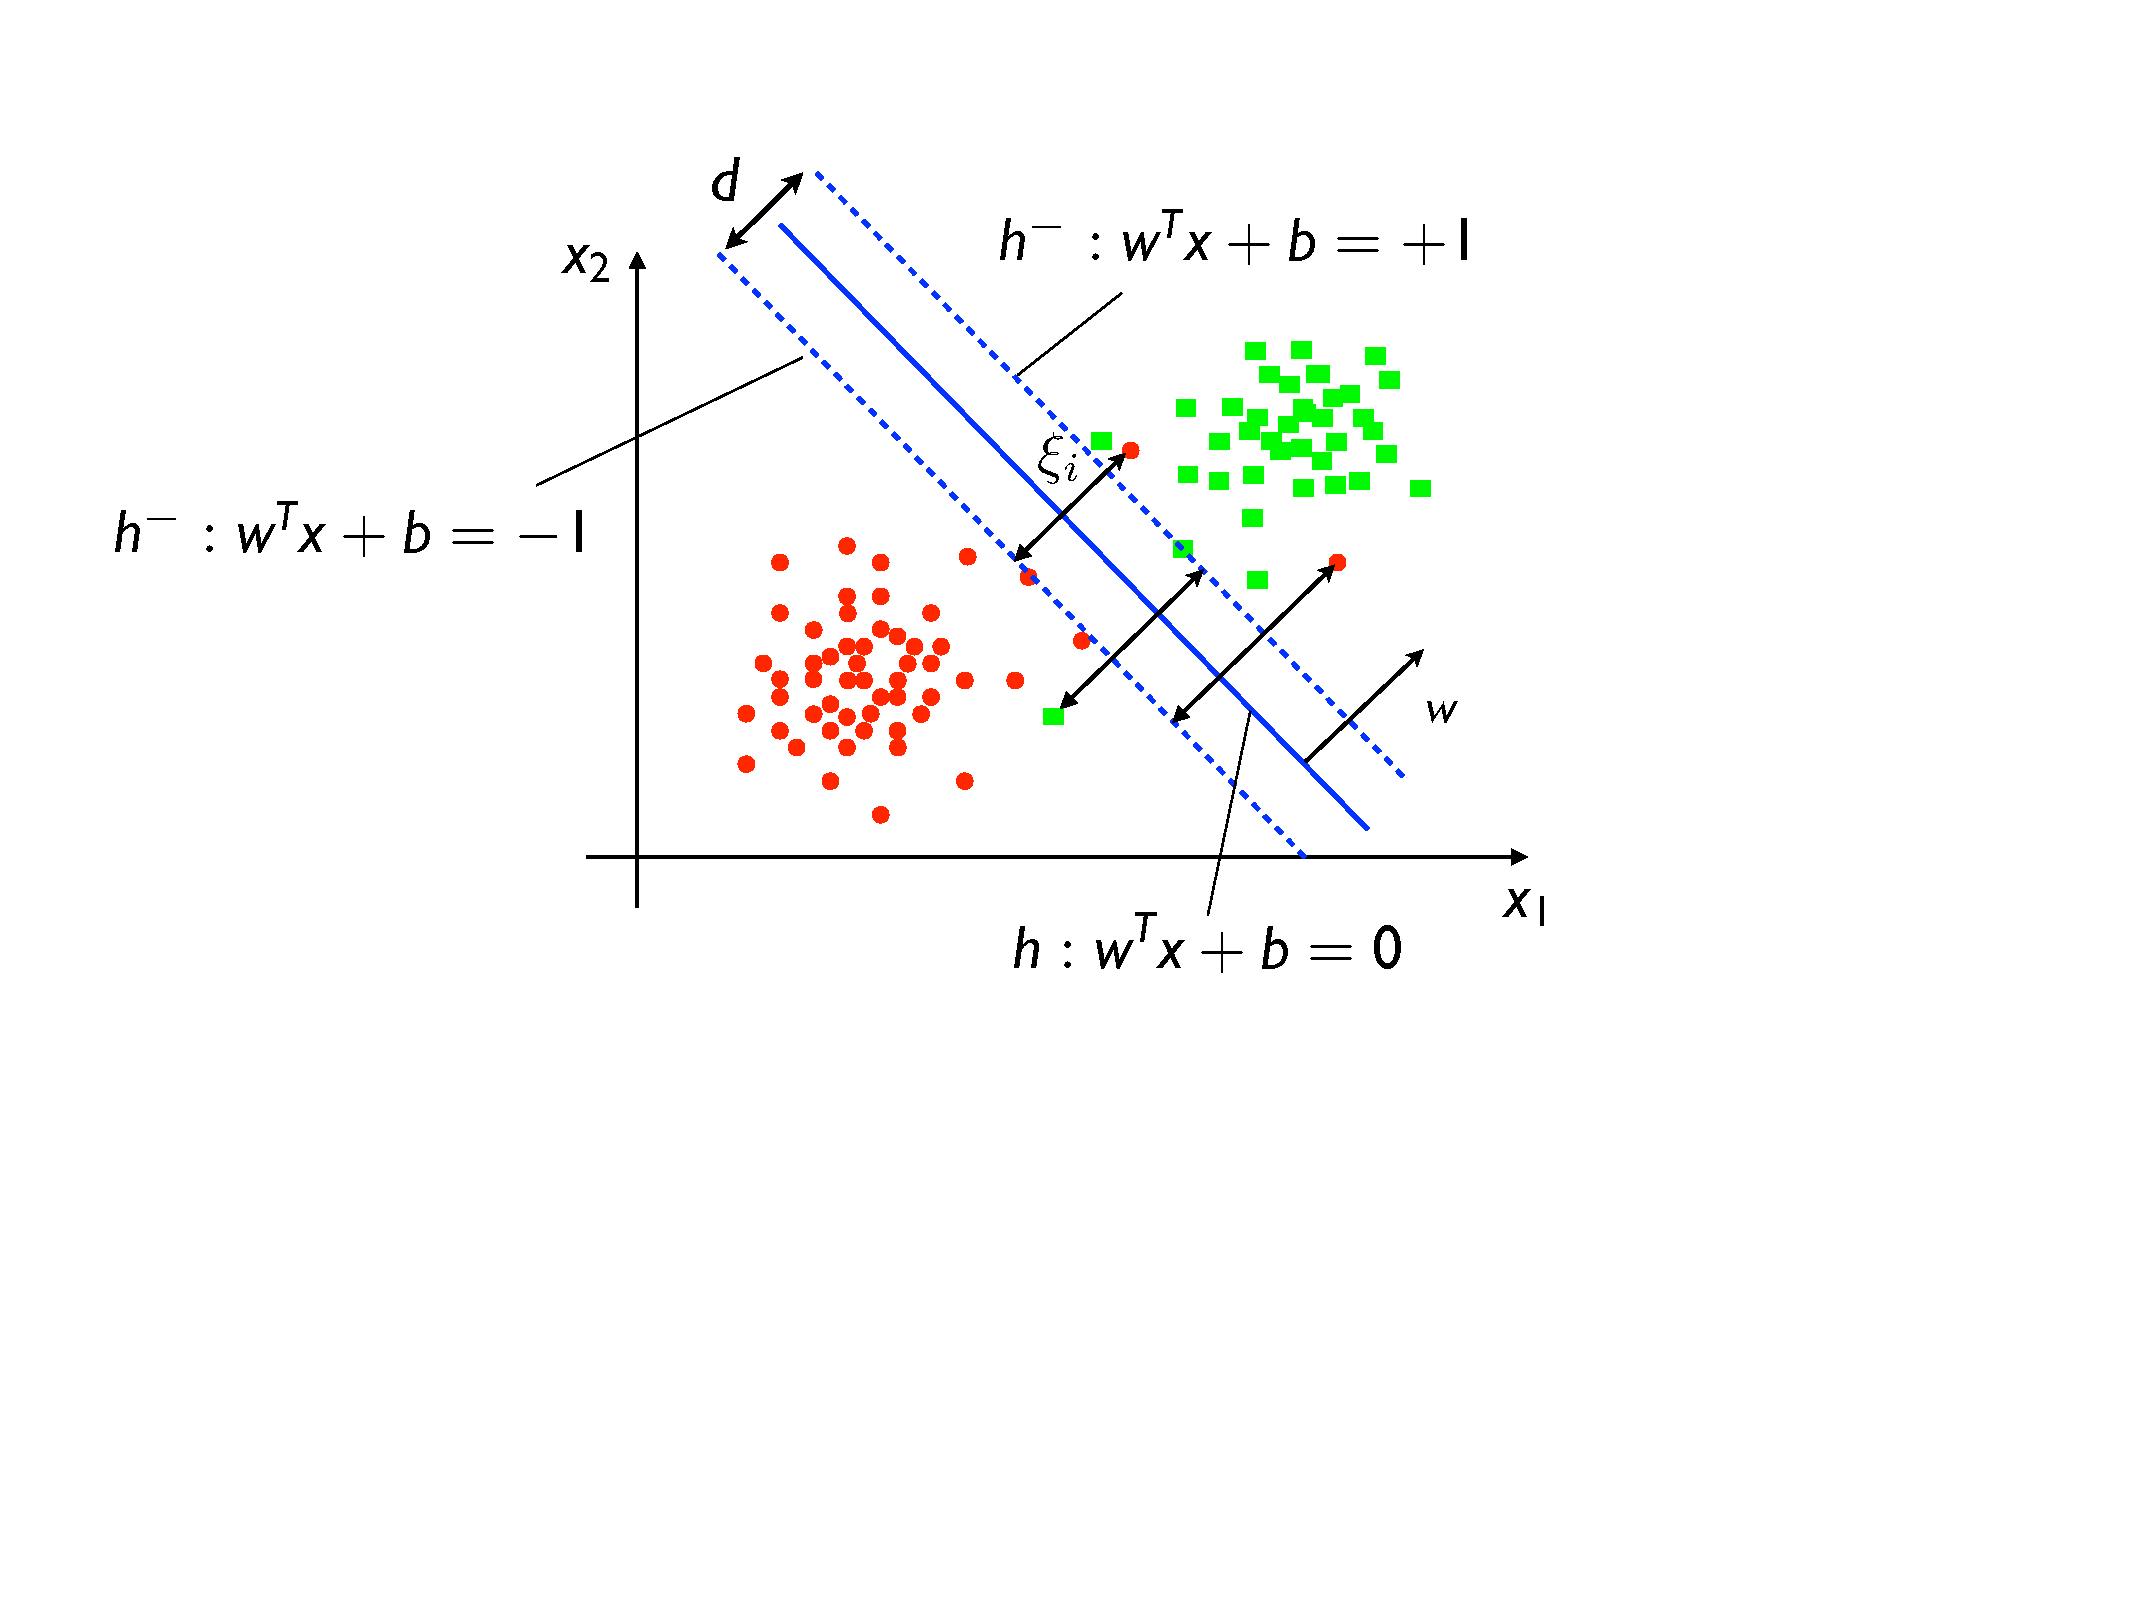
\includegraphics[width=0.6\textwidth]{figures/SVM3.pdf}
  \end{figure}
  \begin{itemize}
    \item Normalement, les données ne sont pas linéairement séparables. 
    \item Dans ce cas, il faut trouver un compromis entre minimiser l'erreur $\sum_{i=1}^{N}L(\langle \wvec, \xvec_i\rangle + b, y_i)$ et minimiser la marge $\|\wvec\|_2^2$. 
    \item Pour la fonction de perte $L$, on choisit l'erreur hinge: 
    \begin{equation}
    L_{hinge}(f(\xvec), y) = \max(0, 1-yf(\xvec)) = \left[1-yf(\xvec)\right]_{+}
    \end{equation}
  \end{itemize}
\end{frame}

\begin{frame}{1.3 SVM pour le cas non-séparable}
  \begin{figure}[htb]
    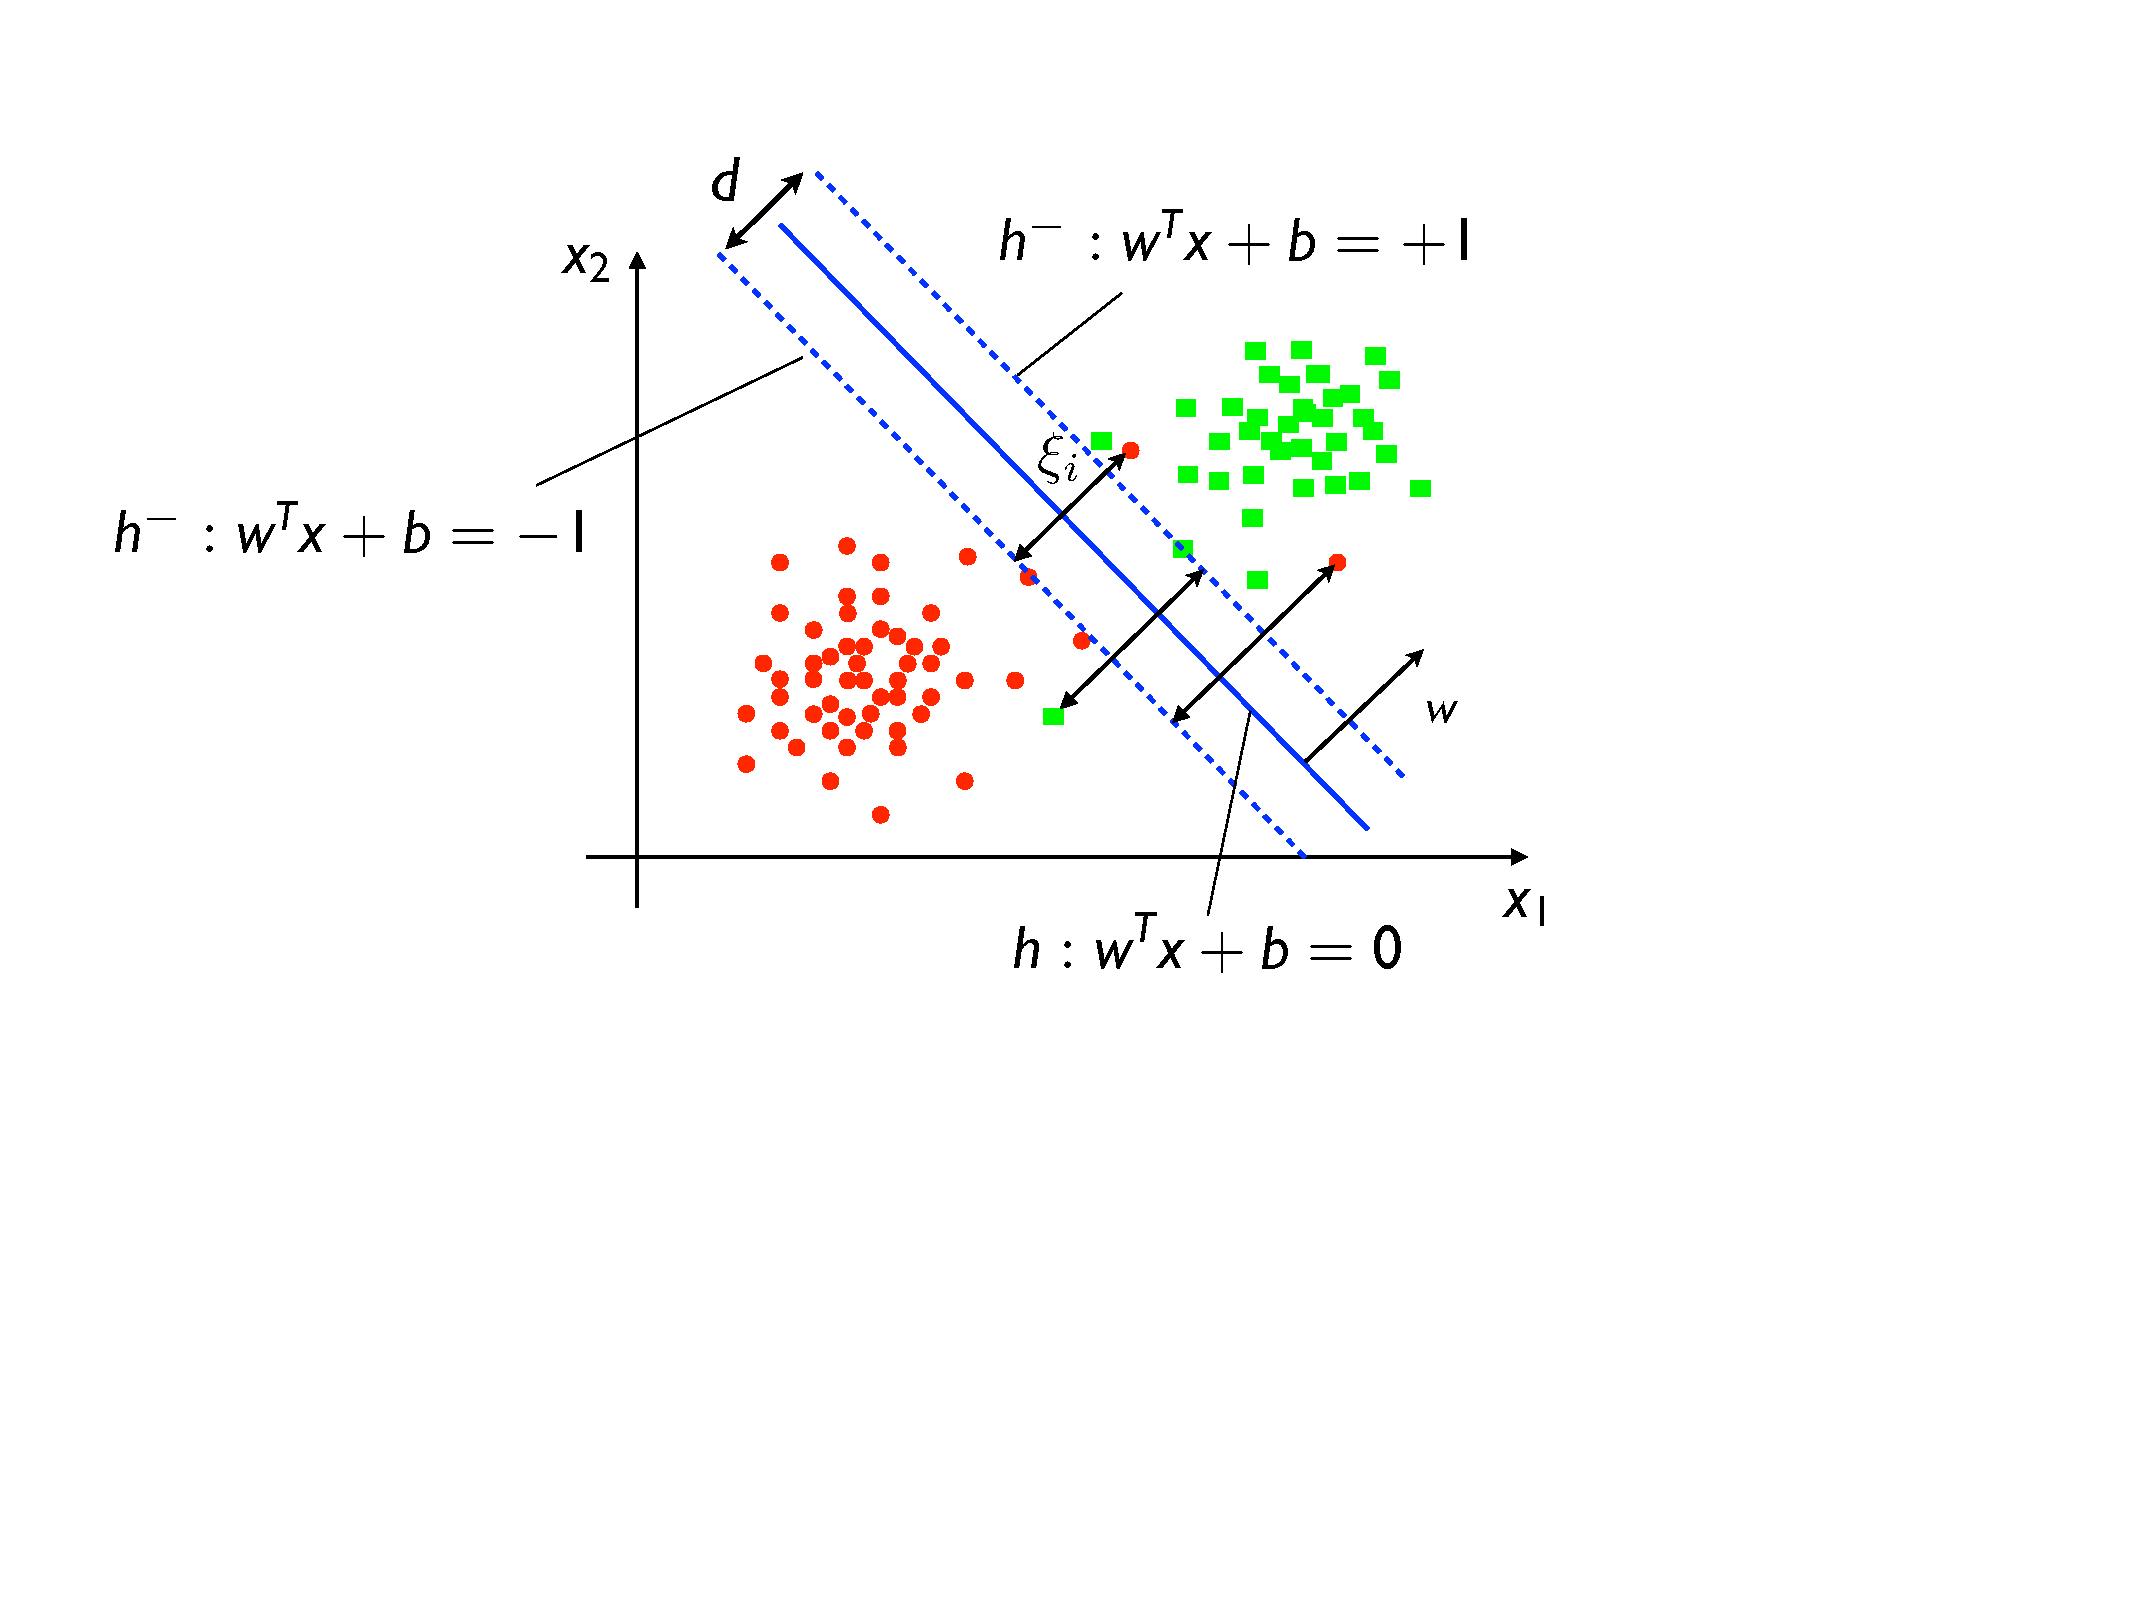
\includegraphics[width=0.6\textwidth]{figures/SVM3.pdf}
  \end{figure}
  \begin{itemize}
    \item On écrit $\xi_i=\left[1-y_if(\xvec_i)\right]_{+}$. 
    \item On a donc : 
    \begin{itemize}
      \item $0<\xi<1$ : classification correcte, mais trop proche de l'hyperplan séparateur
      \item $1<\xi<2$ : classification incorrecte, mais proche de l'hyperplan séparateur
      \item $\xi>2$ : classification incorrecte, loin de l'hyperplan séparateur
    \end{itemize}
  \end{itemize}
\end{frame}

\begin{frame}{1.3 SVM pour le cas non-séparable}
\begin{itemize}
    \item Le problème à minimiser devient donc:
    \begin{eqnarray*}
      \min_{\overrightarrow{w},\xi} & & \frac{1}{2}\|\overrightarrow{w}\|_2^2 + C \sum_{i=1}^{N}\xi_i\\
      \mbox{t.q.} & & y_i(\langle \overrightarrow{w};\overrightarrow{x_i} \rangle + b) \geq 1 - \xi_i \quad i = 1, \ldots, N \\
      & & \xi_i \geq 0 \quad i = 1, \ldots, N
    \end{eqnarray*}
    \item Nous minimisons la somme de deux termes : 
    \begin{itemize}
      \item La somme d'erreurs de classification 
      \item Un terme de régularisation $\|\wvec\|^2$
    \end{itemize}
    \item Maximiser la marge revient à faire une $L_2$ régularisation. 
    \item La solution du problème d'optimisation est similaire au cas précédent. 
\end{itemize}
\end{frame}


\begin{frame}{1.3 SVM pour le cas non-séparable}
\begin{itemize}
    \item Le problème dual s'écrit de façon similaire au cas séparable. 
    \begin{eqnarray*}
 &\max& g(\alphavec) = \sum_{i=1}^{N}\alpha_i - \frac{1}{2}\sum_{i=1}^N\sum_{j=1}^N\alpha_i\alpha_jy_iy_j\langle\xvec_i,\xvec_j\rangle \\
&\mbox{t.q.}& \alpha_i \geq 0 \, \forall i \\
&\, & \alpha_i \leq C \, \forall i \\
&\, & \sum_{i=1}^N\alpha_iy_i=0 
\end{eqnarray*}
\item La seule différence par rapport au cas séparable est la contrainte supplémentaire $\alpha_i \leq C$. 
\item La fonction de décision est toujours donnée par 
\begin{equation}
  f(\xvec) = \sum_{i=1}^N\alpha_iy_i\langle\xvec_i,\xvec\rangle + b 
\end{equation}
\end{itemize}
\end{frame}

% \begin{frame}{Conclusion}
%   \begin{itemize}
%   \end{itemize}
% \end{frame}

% \begin{frame}{1.4 Solution}
%   \begin{itemize}
%     \item La solution du problème d'optimisation implique le formalisme Lagrangian. 
%     \item On obtient une solution pour $\overrightarrow{w}$ : 
%     \begin{equation*}
%       \overrightarrow{w} = \sum_{i=1}^N\alpha_iy_i\overrightarrow{x_i}
%     \end{equation*}
%     ce qui donne l'équation de l'hyperplan : 
%     \begin{eqnarray*}
%       f(\overrightarrow{x}) &=& \sum_{i=1}^N\alpha_iy_i\langle \overrightarrow{x_i}, \overrightarrow{x} \rangle + b\\
%       &=& \sum_{\overrightarrow{x_i} \in SV}\alpha_iy_i\langle \overrightarrow{x_i}, \overrightarrow{x} \rangle + b
%     \end{eqnarray*}
%     \item $SV$ est l'ensemble des vecteurs de support : des vecteurs qui sont situés sur le "ruban". 
%   \end{itemize}
% \end{frame}

% \begin{frame}{1.4 Solution - Observations}
%   \begin{equation*}
%   f = \sum_{\overrightarrow{x_i} \in SV}\alpha_iy_i\langle \overrightarrow{x_i}, \overrightarrow{x} \rangle + b
%   \end{equation*}
%   \begin{enumerate}
%     \item La décision ne dépend que d'un faible nombre d'observations.
%     \item La décision ne dépend que de produits scalaires entre $\overrightarrow{x_i}$ et $\overrightarrow{x}$. 
%   \end{enumerate}
% \end{frame}



\begin{frame}
  \begin{center}
    \large{2. Méthode à noyaux}
  \end{center}
\end{frame}


\begin{frame}
  \frametitle{2.1 Motivation}
  \begin{center}
    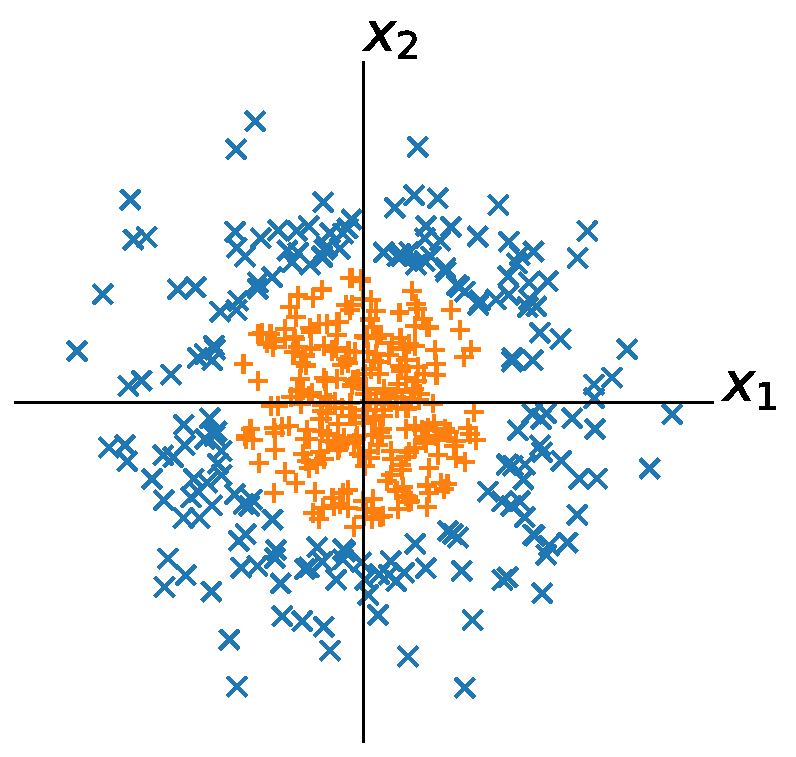
\includegraphics[width=0.4\textwidth]{figures/circular-separable}%
    \hfill
    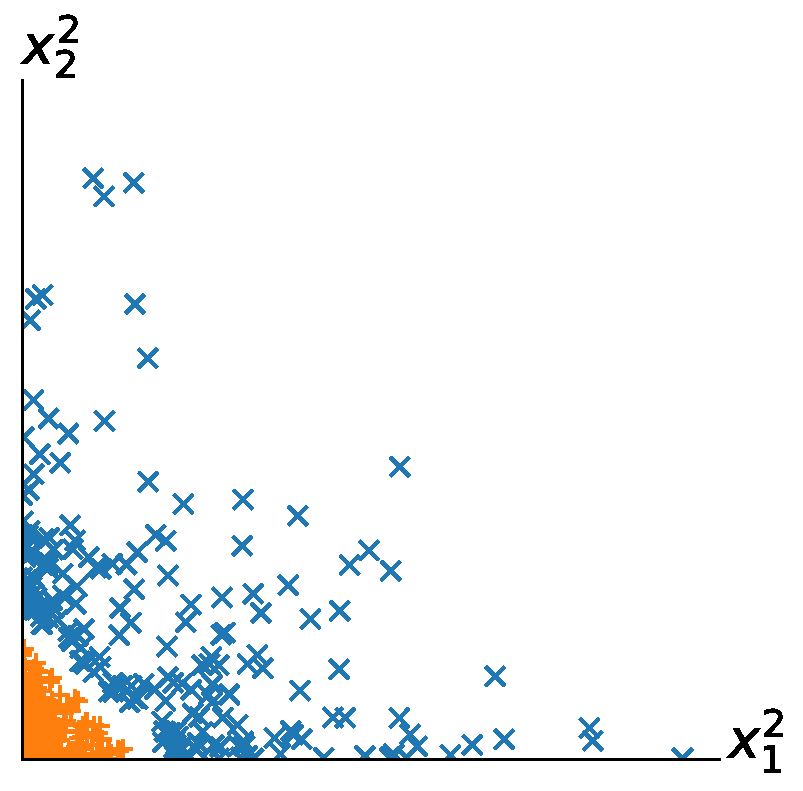
\includegraphics[width=0.4\textwidth]{figures/circular-separable-mapped}%
  \end{center}
  \begin{itemize}
    \item Limitation de SVM: linéarité. 
    \item Extension possible : 
    \begin{enumerate}
      \item transformer les données dans un autre espace (à plus grande dimension)
      \item entrainer / appliquer des SVM dans cet espace. 
    \end{enumerate}
    % \item Dans cet exemple : 
    % \begin{eqnarray*}
    % \phi &:& \RR^2 \mapsto \RR^2 \\
    %      &,& (x_1,x_2) \mapsto (x_1^2, x_2^2) 
    % \end{eqnarray*}
    % les données deviennent alors linéairement séparable. 

%  \item[] $k: (\xvec, \xvec^\prime) \mapsto (1 + \langle \xvec, \xvec^\prime \rangle)^2$
%  \item[] Équivaut à $\varphi : (x_1, x_2, \dots, x_p) \mapsto (1, x_1, \dots, x_p,
%    x_1^2, x_2^2, \dots, x_p^2, \sqrt{2} x_1 x_2, \dots, \sqrt{2}x_{p-1}x_p).$
  \end{itemize}
\end{frame}

\begin{frame}
  \frametitle{2.1 Motivation}
  \begin{center}
    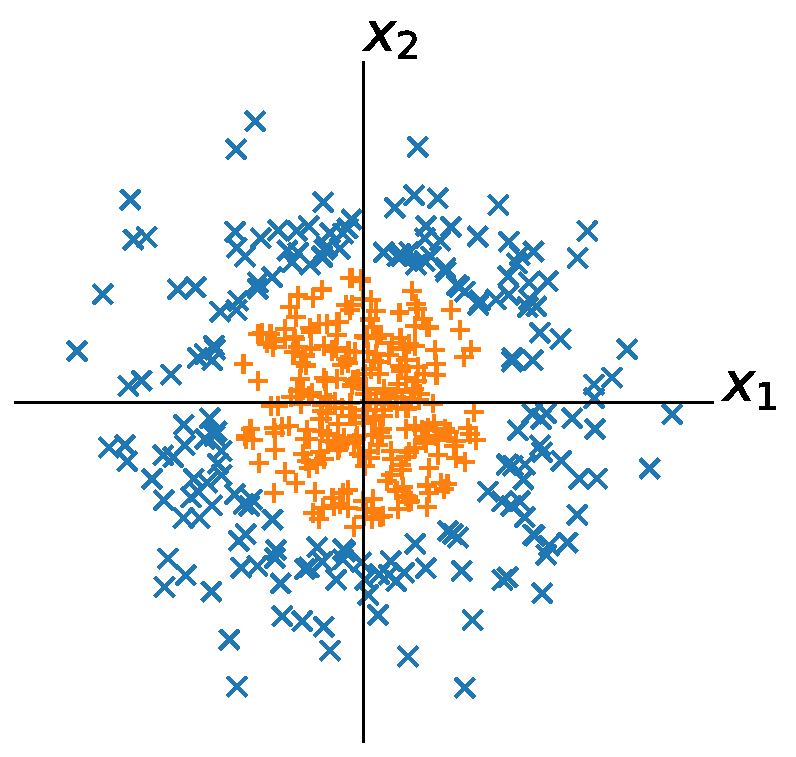
\includegraphics[width=0.4\textwidth]{figures/circular-separable}%
    \hfill
    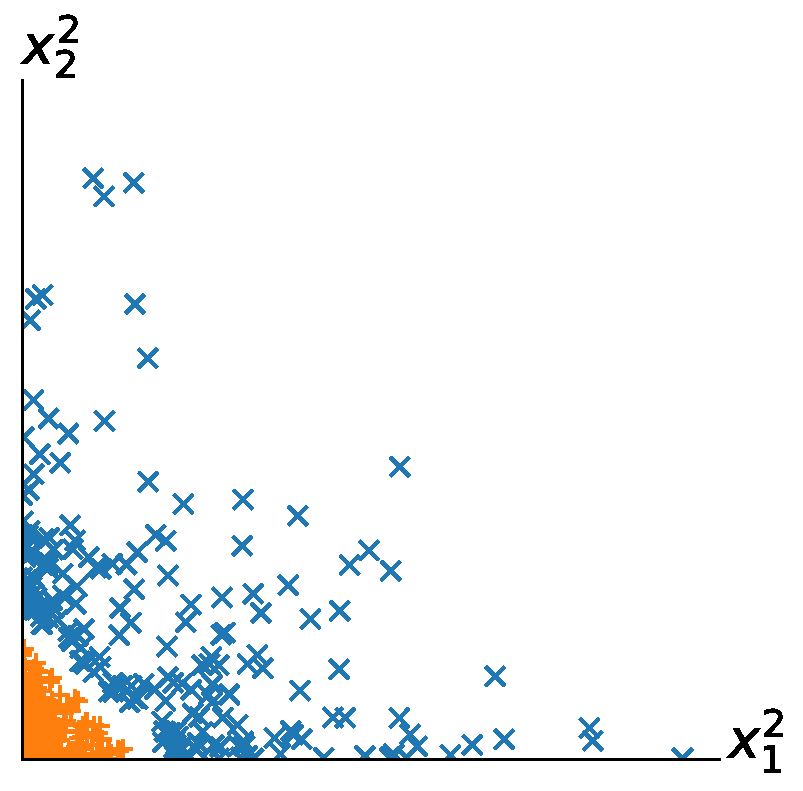
\includegraphics[width=0.4\textwidth]{figures/circular-separable-mapped}%
  \end{center}
  \begin{itemize}
    \item Dans cet exemple : 
    \begin{eqnarray*}
    \phi &:& \RR^2 \rightarrow \RR^2 \\
         &\,& (x_1,x_2) \mapsto (x_1^2, x_2^2) 
    \end{eqnarray*}
    \item Les données deviennent alors linéairement séparable. 
  \end{itemize}
\end{frame}

\begin{frame}
  \frametitle{2.2 SVM à noyau}
  \begin{itemize}
    \item On suppose que nos données sont définies sur un espace quelconque $\xcal$ (e.g. $\RR^p$). 
    \item Nous allons ensuite redécrire les données dans un espace de Hilbert $\hcal$ grâce à une application $\phi$.    
    \begin{eqnarray*}
    \phi &:& \xcal \rightarrow \hcal \\
         &\,& \xvec \mapsto \phi(\xvec) 
    \end{eqnarray*}
  \end{itemize}
\end{frame}

\begin{frame}
  \frametitle{2.2 SVM à noyau}
  \begin{itemize}
    \item Le problème dual devient alors : 
    \begin{eqnarray*}
 &\max& g(\alphavec) = \sum_{i=1}^{N}\alpha_i - \frac{1}{2}\sum_{i=1}^N\sum_{j=1}^N\alpha_i\alpha_jy_iy_j\langle\phi(\xvec_i),\phi(\xvec_j)\rangle \\
&\mbox{t.q.}& \alpha_i \geq 0 \, \forall i \quad
\alpha_i \leq C \,\forall i \quad
\sum_{i=1}^N\alpha_iy_i=0 
\end{eqnarray*}
\item La fonction de décision est toujours donnée par 
\begin{equation}
  f(\xvec) = \sum_{i=1}^N\alpha_iy_i\langle\phi(\xvec_i),\phi(\xvec)\rangle + b 
\end{equation}
  \end{itemize}
\end{frame}

\begin{frame}
  \frametitle{2.2 SVM à noyau}
  \begin{itemize}
    \item Les SVM ne dépendent que des produits scalaires (à l'entrainement et à l'inférence)
    \item Si on sait comment calculer le produit scalaire dans l'espace $\hcal$, on peut ne pas faire la transformation $\phi$ explicitement. 
    \item On parle alors d'astuce de noyau. 
    \item Noyau : 
    \begin{eqnarray*}
    k &:& \xcal \times \xcal \rightarrow \RR \\
      &\,& \xvec, \xvec' \mapsto \langle\phi(\xvec), \phi(\xvec')\rangle_{\hcal}
    \end{eqnarray*}
  \end{itemize}
\end{frame}

\begin{frame}
  \frametitle{2.2 SVM à noyau}
  \begin{itemize}
    \item Avec cela, nous pouvons définir le SVM à noyau
    \begin{eqnarray*}
 &\max& g(\alphavec) = \sum_{i=1}^{N}\alpha_i - \frac{1}{2}\sum_{i=1}^N\sum_{j=1}^N\alpha_i\alpha_jy_iy_jk(\xvec_i, \xvec_j) \\
&\mbox{t.q.}& \alpha_i \geq 0 \, \forall i \quad
\alpha_i \leq C \,\forall i \quad
\sum_{i=1}^N\alpha_iy_i=0 
\end{eqnarray*}
\item La fonction de décision est ensuite donnée par : 
\begin{equation}
  f(\xvec) = \sum_{i=1}^N\alpha^\ast_iy_ik(\xvec_i,\xvec) + b^\ast 
\end{equation}

  \end{itemize}
\end{frame}


% \begin{frame}
%   \frametitle{2.3 Les noyaux}
%   \begin{itemize}

%   \end{itemize}
% \end{frame}


\begin{frame}
  \frametitle{2.3 Les noyaux - Produit scalaire}
  \begin{itemize}
  \item $\langle \xvec, \xvec^\prime \rangle = \sum_{j=1}^p x_j x_j^\prime$
  \item $\langle \xvec, \xvec^\prime \rangle = \ltwonorm{\xvec} \ltwonorm{\xvec^\prime} \cos \theta$ \hspace{1em}
     $\ltwonorm{\xvec}^2 = \langle \xvec, \xvec \rangle$
  \item Interprétable comme \blue{mesure de similarité}
  \item \blue{Forme définie positive bilinéaire :}
    \begin{itemize}
    \item $\langle \xvec, \xvec^\prime \rangle = \langle \xvec^\prime, \xvec \rangle$
      pour tout $\xvec, \xvec^\prime \in \mathcal{X}$
    \item $\langle \xvec + \zvec, \xvec^\prime \rangle = \langle \xvec, \xvec^\prime \rangle +
      \langle \zvec, \xvec^\prime \rangle$       pour tout $\xvec, \xvec^\prime, \zvec \in \mathcal{X}$
    \item $\langle a \xvec, \xvec^\prime \rangle = a \langle \xvec, \xvec^\prime \rangle$ pour tout $a \in \RR$
    \item $\langle \xvec, \xvec \rangle \geq 0$ et $\langle \xvec, \xvec \rangle = 0 \text{ ssi } \xvec = 0$
    \end{itemize}
  \item Apparaît dans de nombreux algorithmes d'apprentissage.
  \end{itemize}
\end{frame}

\begin{frame}
  \frametitle{2.3 Les noyaux - propriétés}
  \begin{itemize}
  \item \blue{Généralisation} du produit scalaire : $k: \xcal \times \xcal \rightarrow \RR$
    \begin{itemize}
    \item \blue{sémantiquement} une similarité
    \item \blue{mathématiquement} une forme définie positive 
    \end{itemize}
  \item Aronszajn: Si $k$ est semi-définie positive\footnote{Pour tout
      $m \in \NN^*$, pour tout
      $\{\xvec_1, \xvec_2, \dots, \xvec_m\} \in \xcal,$ la matrice
      $K \in \RR^{m \times m}$ telle que $K_{il} = k(\xvec_i, \xvec_l)$ est
      semi-définie positive}, il existe un espace de Hilbert $\hcal$ et une application
    $\varphi: \xcal \rightarrow \hcal$ telle que
    $\textcolor{MyOrange}{k(\xvec, \xvec^\prime) = \langle \varphi(\xvec), \varphi(\xvec^\prime)\rangle_{\hcal}}$
    pour tout $\xvec, \xvec^\prime, \zvec \in \mathcal{X}$
  \end{itemize}
\end{frame}

\begin{frame}
  \frametitle{2.3 Les noyaux - Astuce du noyau}
  \begin{itemize}
    \item[]    $\textcolor{MyOrange}{k(\xvec, \xvec^\prime) = \langle \varphi(\xvec), \varphi(\xvec^\prime)\rangle_{\hcal}}$
    \item Si un algorithme ne fait intervenir les éléments de $\xcal$ que dans
      des produits scalaires, \blue{remplacer ces produits scalaires} par $k$ est
      équivalent à appliquer l'algorithme dans $\hcal$ après avoir appliqué
      $\varphi$
    \item Utile \blue{si $k$ est plus simple à calculer que $\varphi$}
      \pause
    \item Exemple : \blue{noyau quadratique}
      $k: (\xvec, \xvec^\prime) \mapsto (1 + \langle \xvec, \xvec^\prime \rangle)^2$
    \item[] Équivaut à $\varphi : (x_1, x_2, \dots, x_p) \mapsto (1, x_1, \dots, x_p,
      x_1^2, x_2^2, \dots, x_p^2, \sqrt{2} x_1 x_2, \dots, \sqrt{2}x_{p-1}x_p).$
  \end{itemize}
\end{frame}

\begin{frame}
  \frametitle{2.3 Les noyaux - Noyau quadratique}
  \begin{itemize}
  \item[] $k: (\xvec, \xvec^\prime) \mapsto (1 + \langle \xvec, \xvec^\prime \rangle)^2$
  \item[] Équivaut à $\varphi : (x_1, x_2, \dots, x_p) \mapsto (1, x_1, \dots, x_p,
    x_1^2, x_2^2, \dots, x_p^2, \sqrt{2} x_1 x_2, \dots, \sqrt{2}x_{p-1}x_p).$
  \end{itemize}
  \begin{center}
    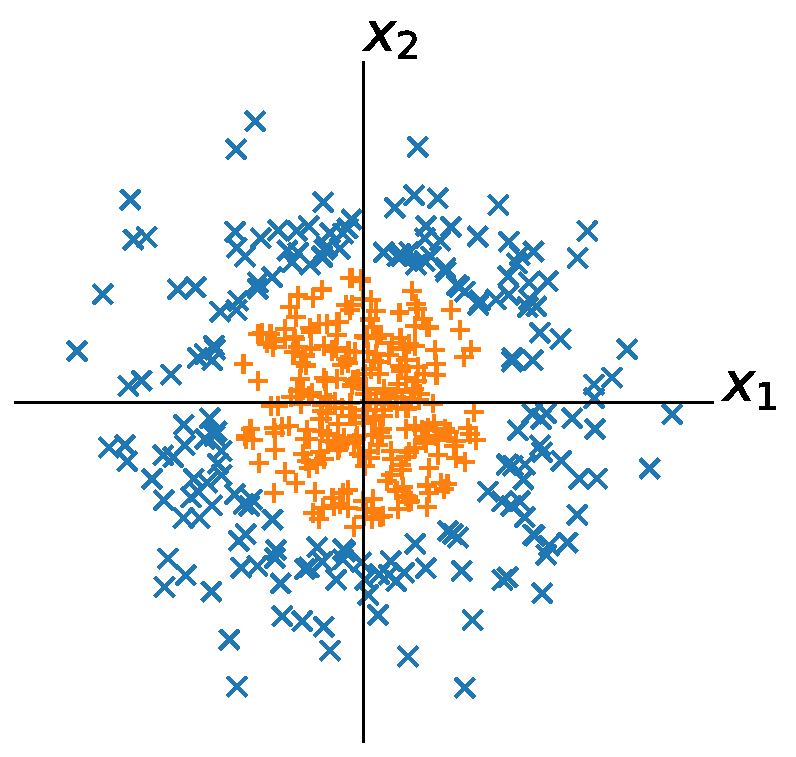
\includegraphics[width=0.4\textwidth]{figures/circular-separable}%
    \hfill
    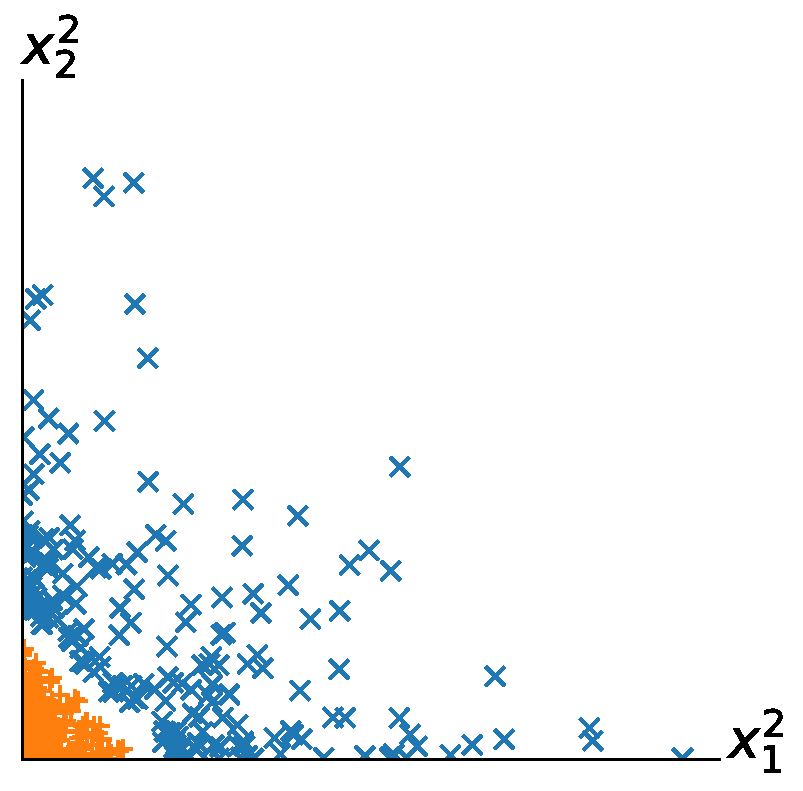
\includegraphics[width=0.4\textwidth]{figures/circular-separable-mapped}%
  \end{center}
\end{frame}

% \begin{frame}
%   \frametitle{1.4 Régression ridge à noyau}
%   \begin{itemize}
%   \item \blue{Régression ridge :}
%     {\footnotesize $\argmin_{\betavec \in \RR^{p+1}} \frac1n \left(\yvec - X \betavec \right)^\top
%       \left(\yvec - X \betavec \right) + \lambda \ltwonorm{\betavec} $}      
%     \begin{itemize}
%     \item Solution : $\betavec^* = \left(X^\top X + \lambda I_p \right)^{-1} X^\top \yvec$
%     \item Modèle : $f: \xvec \mapsto \langle \betavec^*, \xvec \rangle$
%     \end{itemize}
%   \item Reformulation :
%     $f: \xvec \mapsto \textcolor{Aubergine}{\xvec X^\top} \left( \lambda I_n +
%       \textcolor{MyPink}{XX^\top} \right)^{-1} \yvec $
%     \pause
%     \begin{itemize}
%     \item $\textcolor{Aubergine}{\xvec X^\top} \in \RR^n$ a pour $i$-ème entrée :
%       $\textcolor{Aubergine}{\langle \xvec, \xvec_i \rangle}$    
%     \item $\textcolor{MyPink}{X X^\top} \in \RR^{n \times n}$ a pour entrée $(i,l)$ :
%       $\textcolor{MyPink}{\langle \xvec_i, \xvec_l \rangle}$
%     \end{itemize}
%     \pause
%   \item \blue{Kernelization :} remplacer $\textcolor{Aubergine}{\xvec X^\top}$ par
%     $\textcolor{Aubergine}{\kappa} \in \RR^n$ tel que
%     $\textcolor{Aubergine}{\kappa_i = k(\xvec, \xvec_i)}$ et $\textcolor{MyPink}{XX^\top}$ par
%     $\textcolor{MyPink}{K} \in \RR^{n \times n}$ telle que $\textcolor{MyPink}{K_{il} = k(\xvec_i, \xvec_l)}$
%   \item[] équivaut à transformer les données par $\varphi$ puis apprendre une régression ridge, \blue{pour environ le même coût algorithmique}
%   \end{itemize}
% \end{frame}

\begin{frame}
  \frametitle{2.3 Les noyaux - Exemples de noyaux}
  \begin{itemize}
  \item \blue{Noyau quadratique} $k: (\xvec, \xvec^\prime) \mapsto (1 + \langle \xvec, \xvec^\prime \rangle)^2$
  \item[] $\varphi$ calcule tous les monômes de degré au plus 2 de $x_1, x_2, \dots, x_p$ 
    \pause
  \item \blue{Noyau polynomial} $k: (\xvec, \xvec^\prime) \mapsto (1 + \langle \xvec, \xvec^\prime \rangle)^d$
  \item[] $\varphi$ calcule tous les monômes de degré au plus $d$ de $x_1, x_2, \dots, x_p$ 
    \pause 
  \item \blue{Noyau RBF gaussien} $k: (\xvec, \xvec^\prime) \mapsto
    \exp\left( - \frac{\ltwonorm{\xvec - \xvec^\prime}^2}{\sigma^2} \right)$
  \item[] $\varphi$ calcule tous les monômes de $x_1, x_2, \dots, x_p$ 
  et $\hcal$ est de dimension infinie. 
  \end{itemize}
\end{frame}

% \begin{frame}
%   \frametitle{2.3 Les noyaux - Exemples de noyaux}
%   \begin{itemize}
%   \item \blue{Noyau pour chaîne de caractères} $k: (\xvec, \xvec^\prime) \mapsto
%     \sum_{u \in \aset^m} \psi_u(\xvec) \psi_u(\xvec^\prime)$
%     \begin{itemize}
%     \item $\aset^m$ = l'ensemble des chaînes de $m$ caractères sur l'alphabet $\aset$
%     \item $\psi_u(\xvec) = 1$ si $u$ est une sous-chaîne de $\xvec$ et $0$ sinon.
%     \end{itemize}
%   \pause
%   \item $k(\xvec, \xvec^\prime)$ est le nombre de chaînes de $m$ caractères
%     communes à $\xvec$ et $\xvec^\prime$ et peut être calculé en
%     $\mathcal{O}(|\xvec|)$ au lieu de $\mathcal{O}(|\aset|^m)$.
%     \pause
%   \item Si $m=8$, $|\aset|=20$ et en moyenne $|\xvec| = 485,$ on compare 25,6 milliards
%     d'opérations à moins de 500.
%   \end{itemize}
% \end{frame}

\begin{frame}
  \frametitle{Recap : Méthodes à noyau}
  \begin{itemize}
  \item \black{Idée :} Remplacer dans un algorithme tous les \blue{produits scalaires} par des \blue{noyaux}
  \item Apprendre des modèles \blue{non-linéaires} efficacement
  \item Appliquer des modèles linéaires à des \blue{objets} dont la représentation en $p$ dimensions n'est pas évidente (images, protéines, graphes, etc.)
    
  \end{itemize}
\end{frame}

\begin{frame}
  \frametitle{Conclusion: SVM}
  \begin{itemize}
  \item Maximiser la marge revient à régulariser le problème de classification.
  \item Les SVM reposent sur l'optimisation convexe sous contraintes qui est très bien comprise. 
  \item Avec la méthode de noyaux, on a un mécanisme puissant pour passer outre les classifieurs linéaires.
  \item Les SVM fonctionnent bien si le nombre de descripteurs est plus grand que le nombre d'échantillons dans $\dset$. 
  \end{itemize}
\end{frame}

% \begin{frame}
%   \begin{center}
%     \large{2. Machines à vecteurs de support}
%   \end{center}
% \end{frame}

% \begin{frame}[t]
%   \frametitle{2.1 Formulation primale}
%   \begin{itemize}
%   \item Classification binaire, $\ycal = \{-1, 1\}$ 
%     \[\argmin_{\betavec \in \RR^p, b \in \RR} \frac12 \ltwonorm{\betavec}^* + C \sum_{i=1}^n
%       \max\left( 0, 1 - y_i \left( \langle \betavec, \xvec_i \rangle + b \right)\right)\]
%   \end{itemize}
%   \begin{center}
%     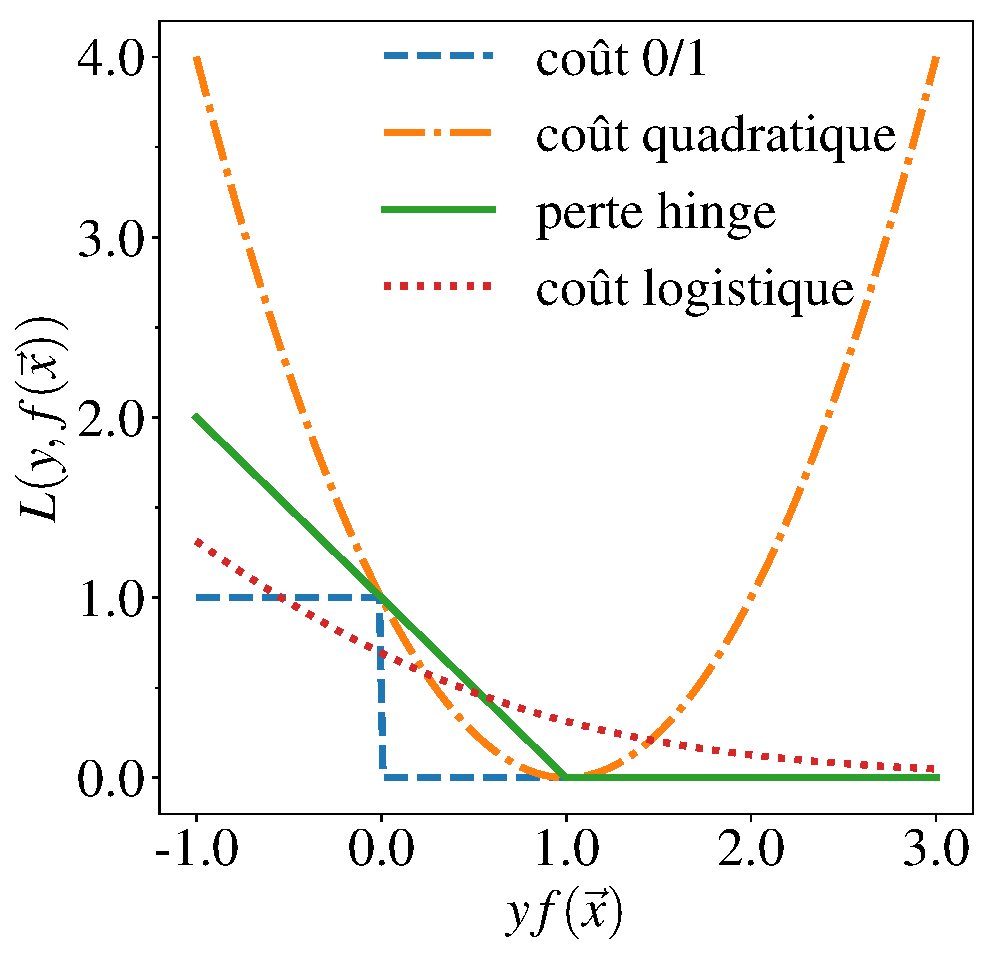
\includegraphics[width=0.5\textwidth]{figures/classif_losses}%
%   \end{center}
% \end{frame}

% \begin{frame}[t]
%   \frametitle{2.1 Formulation primale}
%   \begin{itemize}
%   \item Classification binaire, $\ycal = \{-1, 1\}$ 
%     \[\argmin_{\betavec \in \RR^p, b \in \RR} \frac12 \ltwonorm{\betavec}^* + C \sum_{i=1}^n
%       \max\left( 0, 1 - y_i \left( \langle \betavec, \xvec_i \rangle + b \right)\right)\]
%   \end{itemize}
%   \begin{center}
%     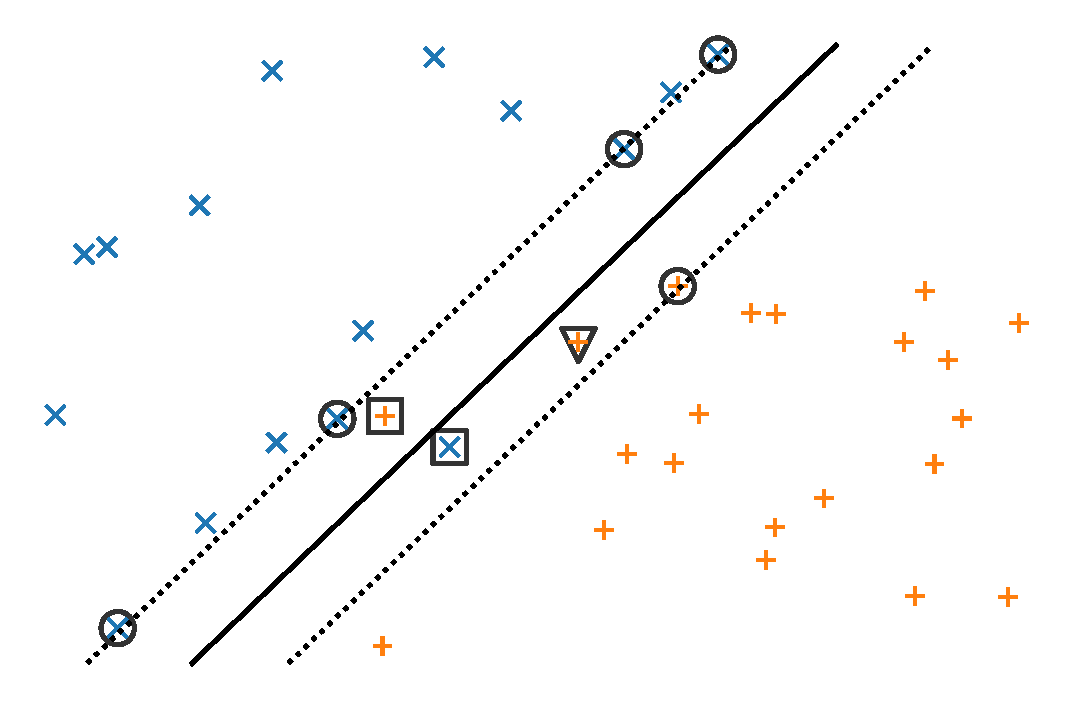
\includegraphics[width=0.7\textwidth]{figures/non-linearly-separable}%
%   \end{center}
% \end{frame}

% \begin{frame}[t]
%   \frametitle{2.2 Formulation duale}
%     {\small \[\argmax_{\alphavec \in \RR^n} \sum_{i=1}^n \alpha_i - \frac12 \sum_{i=1}^n \sum_{l=1}^n
%       \alpha_i \alpha_l y_i y_l \langle \xvec_i, \xvec_l \rangle   \]}
%   \begin{itemize}
%   \item[] sous les contraintes $\sum_{i=1}^n \alpha_i y_i = 0$  et $0 \leq \alpha_i \leq C$ 
%   \item Modèle : $f: \xvec \mapsto \sum_{i=1}^n \alpha_i y_i \langle \xvec_i, \xvec \rangle$
%   \end{itemize}
% \end{frame}

% \begin{frame}[t]
%   \frametitle{2.3 SVR (Support Vector Regression)}
%   \begin{itemize}
%   \item Perte $\varepsilon$-insensible :
%     \[L(y, f(\xvec) = \max(0, |f(\xvec) - y| - \varepsilon)\]
%   \end{itemize}
%   \begin{center}
%     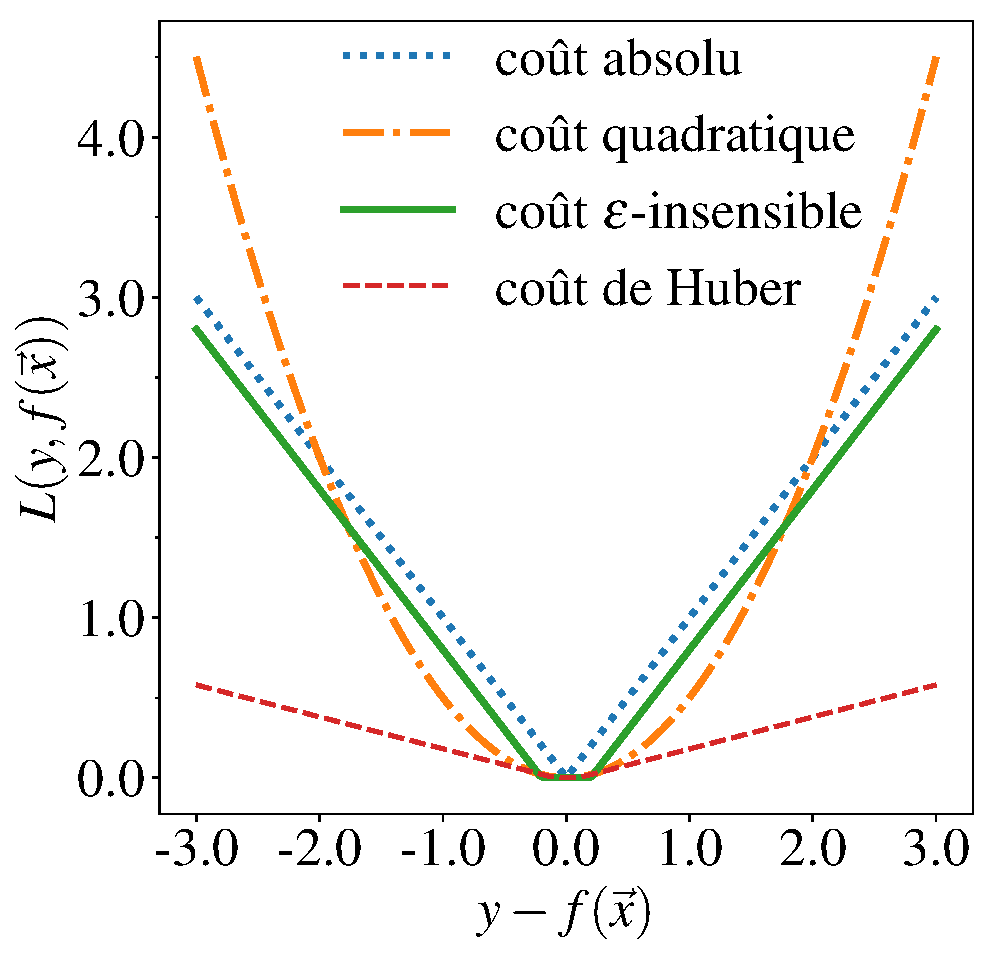
\includegraphics[width=0.5\textwidth]{figures/regression_losses}%
%   \end{center}
% \end{frame}
